% !Mode:: "TeX:UTF-8"
% 此文件从2019.10.18开始写作

\chapter{牛顿引力与狭义相对论}\label{chsr}

之前各章节讲述的几乎是纯数学,自然采取处处以数学为中心的方式来叙述问题.
从本章开始讲述物理,我们将以物理为中心来讲述,把数学当成工具;
我们也会进一步解释之前章节中有关物理的定义等.



时间和空间是物质的基本属性,与人们生活息息相关,
也是物理学的最基本概念.
狭义相对论是关于时间和空间的理论,它不涉及动力学,只是运动学的理论;
然而这一理论管理着除了引力之外的所有物理学,所以学习狭义相对论是
认知理论物理不可或缺的基础知识.

本章内容不是自足的,只是回顾了一些我认为重要的内容.
我们假定读者已熟悉采用$1+3$分解方式的狭义相对论;
可参阅文献\parencite[Ch.1]{landau_2-classical-fields}、
\parencite[Ch.11]{jackson1998}、\parencite{liu_fei2008}等.

本章大体安排:先讨论惯性系定义; 
接着回顾伽利略变换和牛顿万有引力;
继而回顾爱氏的狭义相对论基本原理;
然后回顾相对论力学以及匀加速运动;
之后回顾麦克斯韦方程组;
这几节采用$1+3$分解方式叙述,纯空间矢量采用黑体字符表述.
直到\S\ref{chsr:sec_spacetime-structure-Min},
开始采用四维语言来重新描述狭义相对论.



\section{惯性参考系定义刍议}\label{chsr:sec_inertialframe}

这一小节我们讨论一下惯性系\index[physwords]{惯性参考系}的定义,
结论仍是开放性的.

\index[physwords]{狭义相对论}

\index[physwords]{惯性系} \index[physwords]{惯性定律}



一般认为牛顿第一定律定义了惯性系,即,当质点所受合外力为零时,
质点所在的静止或作匀速直线运动的参考系,称为惯性系.例如
参见\textcite[\S 1]{landau_2-classical-fields}.

然而这个定义是有疑问的!什么是“所受合外力为零”,如何判定?
在牛顿力学范畴内恐怕只能说:如果质点保持匀速直线运动或静止,
则所受合外力为零.这是循环定义,显然是不合适的;
所以在牛顿力学范畴内无法确切定义惯性系.

阿尔伯特$\cdot$爱因斯坦\cite[p.58]{einstein1950}对此作了很好的总结:
\begin{quotation}
    {\textsf{
    The weakness of the principle of inertia lies in this,
    that it involves an argument in a circle: a mass moves
    without acceleration if it is sufficiently far from other bodies;
    we know that it is sufficiently far from other bodies
    only by the fact that it moves without acceleration. }}

    {\fangsong 译文:惯性原理的缺点在于,它涉及到一个循环论证:
        如果质点离其它物体足够远,那么此质点作无加速度运动;
        我们知道只有质点作无加速度运动时,才可确认它离其它物体足够远.}
\end{quotation}
我们的描述只不过把,爱因斯坦的“离其它物体足够远”,换成了“合外力为零”.

牛顿\index[persons]{牛顿}本人似乎也注意到这个循环逻辑,所以
他引入了“绝对空间”(以太)来定义惯性系.他说,
在宇宙的深处,存在一个绝对静止不动的以太,
相对以太静止或作匀速直线运动的参考系是惯性系.
但以太是不存在的,所以不能这样定义惯性系.

%有人认为宇宙总质心绝对静止不动,这可能是新的以太,找不到可操作性办法
%来寻觅这个总质心;况且宇宙不是平直的.

\index[physwords]{循环定义}

笔者学识范畴之内的观点是:在整个理论体系根基的地方,很多概念是不清楚的,
至少有两个或两个以上的概念不清楚.否则就已经建立起公理体系.
在根基的地方,相互定义、{\kaishu 循环}逻辑恐怕是无法避免的.
惯性系的定义就属于此类.

既然循环逻辑无法避免,那么把这个循环逻辑放在牛顿第二定律更好一些,
即,符合牛顿第二定律的参考系是惯性参考系.
这样,有了惯性系定义,第二定律就成立了,那么当质点所受合外力$F=0$时,
质点加速度$a=0$,也就是意味着质点作匀速直线运动或者静止;
惯性定律就成了第二定律的推论.这使基本物理定律更加精简,没有冗余.
{\footnote{\textcite[p.114]{weinberg_ew-2015}把第一定律看成第二定律的推论.
        原文:This was already known to Gassendi and Huygens.
        It is not clear why Newton bothered to include it as a separate law,
        since the first law is a trivial (though important) consequence of the second.
        译文:(第一定律)早已被伽桑狄和惠更斯所知晓.
        因为第一定律是第二定律的一个显然(但很重要)的推论,
        我不清楚为什么牛顿还费尽心思地把它当成一条独立的定律.

    读者应该能够看出,牛顿最初用以太定义了惯性系,那么,牛顿第二定律就已成立.
    此时,牛顿第一定律便是第二定律的一个特例.这正是Weinberg质疑牛顿的原因.
}}
同时使这个{\kaishu 循环逻辑}更加明显,以引起读者注意到这个悬而未决的问题.

{\kaishu 虽然我们无法准确定义惯性系,但需要假设它的存在,至少局部存在;
    并且需要假设(在局部范围内)时间是均匀流逝的,空间是均匀、各向同性的\cite[\S 3]{landau_1-mechanics}.}


\section{牛顿力学回顾}

\index[physwords]{伽利略变换}

\subsection{伽利略变换}\label{chsr:sec_Galileo}
在相对论发现之前的经典物理学
(牛顿力学)认为时间和空间相互独立,没有任何关系;在宇宙深处
存在一个绝对静止的参考系,这个绝对静止的参考系具有特殊地位.
这就是牛顿的绝对时空观.
这在低速、低能的宏观领域是非常非常精确的近似.

\begin{figure}[htb]
    \centering
    \begin{tikzpicture}
        \draw [-latex] (0,0)--(3.5,0) node[below ] { $x(x')$};
        \draw [-latex] (0,0)--(0,3.0) node[above ] {$y$};
        \draw [-latex] (1,0)--(1,3.0) node[above ] {$y'$};
        \draw [-latex] (0,0)--(-1.5,-1.5) node[above ] {$z$};
        \draw [-latex] (1,0)--(-0.5,-1.5) node[above ] {$z'$};
        \node at (0,-0.3)  {$O$};
        \node at (1.2,-0.3)  {$O'$};
        \node at (0.7,1.5) {$v$};
        \draw[-latex] (0.5,1.3) -- (0.9,1.3);
    \end{tikzpicture}
    \caption{惯性系$O$与$O'$的坐标关系}\label{chsr:pic_oop}
\end{figure}


当麦克斯韦统一电与磁之后,牛顿的经典时空观与电磁理论、实验都
产生了明显的不符.
在牛顿力学中,大家都学过伽利略变换.\index[persons]{伽利略}
设有一个惯性参考系$O$,其中有坐标系$O-xyz$;
另一个惯性参考系$O'$,其中有坐标系$O'-x'y'z'$,见图\ref{chsr:pic_oop};
两参考系有恒定的速度差$\boldsymbol{v}=v \boldsymbol{e}_x$,即方向平行于$x$轴;
在$t=0=t'$时刻,两个系的原点重合,相应坐标轴分别平行且同向,
则两个参考系的变换关系就是伽利略变换
\begin{equation}\label{chsr:eqn_galileo-trans-x}
    x' = x -vt, \quad
    y' = y, \quad
    z' = z, \qquad
    t' \equiv t.
\end{equation}
它的微分形式:
\begin{equation}\label{chsr:eqn_galileo-trans-dx}
	{\rm d}x' = {\rm d}x -v {\rm d}t, \quad
	{\rm d}y' = {\rm d}y, \quad
	{\rm d}z' = {\rm d}z, \qquad
	{\rm d}t' \equiv {\rm d}t.
\end{equation}
伽利略的速度变换是
\begin{equation}\label{chsr:eqn_galileo-trans-vel}
    u'_x = u_x -v, \quad
    u'_y = u_y, \quad
    u'_z = u_z.
\end{equation}
其中
\begin{equation}\label{chsr:eqn_3-Velocity}
  \boldsymbol{u}=\frac{{\rm d} \boldsymbol{x}}{{\rm d}t}, \quad   \boldsymbol{u}'=\frac{{\rm d} \boldsymbol{x}'}{{\rm d}t'} .
\end{equation}
分别表示$O$系和$O'$系中质点的速度,注意与两惯性系间相对速度$\boldsymbol{v}$的区别.




当把伽利略变换用到光速时会有矛盾.比如某运动员在踢足球,足球从他的脚飞出来后
具有速度$v$,那么从他脚上反射的光速是$c$,而从足球上反射的光速是$v+c$;这样
因足球上出来的光先到你的眼睛里,脚上出来的光后到你的眼睛里,故你先看到足球从
他的脚上飞出来,再看到他的脚踢球.因果关系颠倒了!

还有很多其它实验与伽利略变换不符,可参阅文献\parencite{jackson1998,liu_fei2008,zhangyz-2023}相应章节.




\subsection{牛顿引力论}\label{chsr:sec_Newton-Gravity}

设有物体$A$,总质量是$M$,其密度分布是$\rho(y)$;物体$B$总质量是$m$,
处于空间中$\boldsymbol{x}$位置.牛顿万有引力公式为:
\begin{equation}\label{chsr:eqn_Newton-gravity}
    \boldsymbol{F} = -\frac{G M m}{r^2} \hat{\boldsymbol{r}}
    = -Gm   \int \frac{\rho(\boldsymbol{y})}{|\boldsymbol{x}-\boldsymbol{y}|^2}\hat{\boldsymbol{r}} {\rm d}^3y
    =m \nabla_x \int \frac{G \rho(\boldsymbol{y})}{|\boldsymbol{x}-\boldsymbol{y}|} {\rm d}^3y .
\end{equation}
其中$G$是引力常数,$r=|\boldsymbol{x}-\boldsymbol{y}|$是两物体间距离,
$\hat{\boldsymbol{r}}$是两个物体间距离的单位位矢.
上式第三个等号利用了矢量公式$\nabla\frac{1}{r}=-\frac{1}{r^2} \hat{\boldsymbol{r}}$.
我们定义引力势$\Phi$如下:
\begin{equation}\label{chsr:eqn_Newton-gravity-potential}
    \Phi\overset{def}{=} -\int \frac{G \rho(\boldsymbol{y})}{|\boldsymbol{x}-\boldsymbol{y}|} {\rm d}^3y.
     \qquad \text{明显有}\     \boldsymbol{F} = -m \nabla_x \Phi.
\end{equation}
再利用公式$  {\nabla ^2}\frac{1} {  r} =  -4\pi\delta^3 (\boldsymbol{r} )$,
可将牛顿万有引力定律表示成另外一种形式:
\begin{equation}\label{chsr:eqn_Newton-gravity-phi}
    \nabla ^2 \Phi(\boldsymbol{x}) = 4 \pi G \rho(\boldsymbol{x}) .
\end{equation}

连续物质的自引力能为:
\begin{equation}\label{chsr:eqn_NG-self}
    E_{\rm self} = -\frac{1}{2} G \int \frac{ \rho(\boldsymbol{x}) \rho(\boldsymbol{y}) }
    {|\boldsymbol{x}-\boldsymbol{y}|} {\rm d}^3y {\rm d}^3x .
\end{equation}
若物质分布在有限区域,通过Gauss散度定理可将上式改写为:
\begin{equation}\label{chsr:eqn_NG-self-sfb}
    E_{\rm self} = \frac{1}{8\pi G} \int (\nabla \Phi)^2 {\rm d}^3x 
    + \int \rho \Phi {\rm d}^3x  .
\end{equation}
对上式可作如下解释:$\frac{1}{8\pi G} (\nabla \Phi)^2$可看作引力场的能量密度,
$\rho \Phi$可看作引力场和物质相互作用的能量密度.这种解释与静电场非常相似.


\begin{example}\label{chsr:exm_gem}
    电磁力与引力量级差别.
\end{example}

我们用两个质子间的万有引力和库仑力相比来看它们的差别:
\begin{align}
    \frac{F_e}{F_g}=\frac{e^2}{4\pi \epsilon_0 r^2}\cdot \frac{r^2}{Gm^2_p} 
%    = \frac{(\num{1.60d-19})^2} {12.56 \times \num{8.85d-12}\times \num{6.67d-11} \times (\num{1.67d-27})^2}
    \approx 3\times 10^{36} .
\end{align}
再举个形象的例子,读者你拿一块磁铁去吸引桌面上的一个小铁钉,唰的一下就吸起来了;
可见一块磁铁的电磁力便可抵抗整个地球的引力.\qed


\subsection{潮汐力}


\begin{figure}[htb]
    \centering
    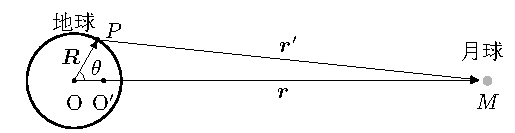
\includegraphics[width=10cm]{fig/II1-Earth.pdf}
    \caption{地月潮汐力} \label{chsr:fig_tidal-force}
\end{figure}



参见图\ref{chsr:fig_tidal-force}.
地心到月心距离为$r$,地球半径为$R$,月球质量为$M$.其中$O'$是地月质心,地球、月球分别绕$O'$点旋转.
我们以地心$O$为原点建立一个坐标系;$z$轴沿地心、月心连线,指向月心方向;
$x$轴在纸面上,垂直于$z$轴,方向向上;按右手叉乘规则确定$y$轴,即垂直于纸面向外.
现在我们来推导地月系统中引潮力的公式.
我们假设地球表面被海水覆盖;
在地球表面$P$点处有质量为$m$的海水质团,质团$m$受月球的吸引力为
\begin{equation}
    \boldsymbol{f} =\frac{GMm}{r^{\prime 3}} \boldsymbol{r}^{\prime} .
\end{equation}

地心坐标系$O-xyz$并非惯性系,需要附加上惯性力之后才能继续用牛顿第二定律.然而,
任何质量在地心参考系内所受的惯性力,等于把它放在地心处时所受引力的负值,二者是精确抵消的.故
\begin{equation}
    \boldsymbol{f}_{I}=-\frac{GMm}{r^3} \boldsymbol{r} .
\end{equation}
引力$\boldsymbol{f}$ 与 惯性力$\boldsymbol{f}_{I}$合力便是{\heiti 潮汐力}$\boldsymbol{f}_{T}$:
\begin{equation}
    \boldsymbol{f}_{T}=\boldsymbol{f}+\boldsymbol{f}_{I}
    =GMm \left(\frac{\boldsymbol{r}^{\prime}}{r^{\prime 3}} -\frac{\boldsymbol{r}}{r^3}\right) .
\end{equation}
从图\ref{chsr:fig_tidal-force}可以看出:$\boldsymbol{r}^{\prime}=\boldsymbol{r}-\boldsymbol{R}$,则有
\begin{equation}
    \frac{1}{r^{\prime 3}}=\left(r^2+R^2-2 r R \cos \theta\right)^{-3/2}
    \approx  \frac{1}{r^{3}}\left(1+ 3\frac{R}{r}\cos\theta \right) .
\end{equation}
已用$R\lll r$,并微扰展开.同时还有
\begin{equation}
    (\boldsymbol{r}-\boldsymbol{R})_z = r-R \cos \theta, \qquad
    (\boldsymbol{r}-\boldsymbol{R})_x = -R \sin \theta .
\end{equation}
故有
\begin{align}
    \left(f_{I}\right)_z =& \frac{GMm}{r^2}\left[\frac{1-\frac{R}{r} \cos \theta}
    {\left(1-\frac{2 R}{r} \cos \theta+\frac{R^2}{r^2}\right)^{3 / 2}}-1\right] 
    \approx \frac{2 GMm}{r^3} R \cos \theta, \label{chsr:eqn_Tidal-Fz} \\
    \left(f_{I}\right)_x \approx & -GMm R \sin \theta \frac{1}{r^{3}}\left(1+ 3\frac{R}{r}\cos\theta \right)
    \approx -\frac{GMm}{r^3} R \sin \theta .
    \label{chsr:eqn_Tidal-Fx}
\end{align}
海水$P$所受潮汐力在$y$方向上为零.
%需注意:以上两式中$R$为地球的半径$R_{\oplus}$,$r$为地月距离$r_{\text {月 }}$.

这个潮汐力具有绕$z$轴旋转的对称性,故$x$、$y$方向是平权的;
我们通过这种对称性导出潮汐力更一般的公式.
\setlength{\mathindent}{0em}
\begin{align*}
    \boldsymbol{f}_T = \boldsymbol{e}_x \left(f_{I}\right)_x + \boldsymbol{e}_y \left(f_{I}\right)_y
    + \boldsymbol{e}_z \left(f_{I}\right)_z
    = \frac{GMm}{r^3}  \left( -\boldsymbol{e}_x R \sin\theta + \boldsymbol{e}_y \times 0
    + \boldsymbol{e}_z 2 R \cos \theta \right).
\end{align*}\setlength{\mathindent}{2em}
海水质团$P$在地球表面;我们已经建立坐标系$O-xyz$,那么$R \cos \theta$便是
质团$P$的$z$坐标分量;$R \sin\theta$是$P$的$x$坐标分量;
如果我们再引入一个方位角$\varphi$,利用绕$z$的对称性,容易得到:
\begin{equation}\label{chsr:eqn_Tidal-Force}
    \begin{aligned}
    \boldsymbol{f}_T =& \frac{GMm}{r^3}  \left( -\boldsymbol{e}_x R \sin\theta \cos\varphi
    - \boldsymbol{e}_y  R \sin\theta \sin\varphi
    + \boldsymbol{e}_z 2 R \cos \theta \right) \\
    =&\frac{GMm}{r^3}  \left( -\boldsymbol{e}_x x - \boldsymbol{e}_y  y
     + \boldsymbol{e}_z 2 z \right) .
    \end{aligned}
\end{equation}
上式第二行中$x$、$y$、$z$是海水质团$P$在我们所建地心坐标系$O-xyz$中的分量.
从上式可以看出地球表面离月亮最远点和最近点的潮汐力大小是相等的,但方向相反,
最远点指向背离月心方向,最近点指向月心方向.这样,沿月心、地心连线方向,
地球表面海水被拉伸了.从上式还可看出,在垂直于月心、地心连线方向,
潮汐力是指向地心的,故在这个方向海水被压缩.

$r$是月心到地心距离,在$O-xyz$系中不难求得
\begin{equation}
    \frac{\partial^2 r^{-1}}{\partial x^2 } =-\frac{1}{r^3} =\frac{\partial^2 r^{-1}}{\partial y^2 } ,
    \quad \frac{\partial^2 r^{-1}}{\partial z^2 } = \frac{2}{r^3}.
    \quad \text{其它二次偏导为零}
\end{equation}
上述偏导皆在地心处取值.由此可知,式\eqref{chsr:eqn_Tidal-Force}可改写为引力势形式
\begin{equation}
    {f}_T^k = -m x^l  \frac{\partial^2 \Phi }{\partial x^l \partial x^k} .
    \qquad \Phi = -\frac{G M }{r} 
\end{equation}
命
\begin{equation}\label{chsr:eqn_Ri00k}
    R_{\hphantom{i}00k}^i  \equiv - \frac{\partial^2 \Phi }{\partial x^i \partial x^k}.
\end{equation}
额外的指标“00”是为了以后对比所用(见\S\ref{chsch:sec_GDTF}).故有
\begin{equation}\label{chsr:eqn_TF-R}
    f^i_T =  m R_{\hphantom{i}00k}^i x^k .
\end{equation}


\begin{example}
    月球、太阳对地球潮汐力比值.
\end{example}
虽然式\eqref{chsr:eqn_Tidal-Force}是以地月系为模型推导得来,
但这个公式适用于任何场合的潮汐力(牛顿力学范畴内).
已知:太阳质量 $M_{s}=1.988\times 10^{30}  $ \si{kg} ,
日地平均距离 $r_s= 1.496\times 10^{11} $ \si{m} ;
月球质量$M_{m} =7.342\times 10^{22}$ \si{kg},地月平均距离$r_m=3.844 \times 10^8$ \si{m}.
两个潮汐力比值为
\begin{equation}
    \frac{f^{\text{日}}_T}{f^{\text{月}}_T} = \frac{ M_s/r_s^3 }{M_m/r_m^3}
    \approx 0.46 = 46 \% .
\end{equation}
上述计算说明太阳对地球的潮汐力大约是月球对地球的一半. \qed

\begin{example}\label{chsr:exam_Roche}
    洛希极限(\'{E}douard Roche,法国天文学家,1820-1883).
\end{example}
一颗质量为$m$、半径为$r$的球形固态星体,
围绕着一颗质量为$M$、半径为$R$的星体作圆周运动.
当$m$的轨道半径小于$r_{\rm cirt}$时,$m$上的小石块将被潮汐力提起;
$r_{\rm cirt}$被称为洛希极限或洛希半径.
只需用式\eqref{chsr:eqn_Tidal-Force}中的$z$分量即可
\begin{equation}\label{chsr:eqn_Roche}
    \frac{2r GM m' }{r^3_{\rm cirt}} =  \frac{ Gm m' }{r^2}
    \ \Rightarrow \ 
    r_{\rm cirt} = r \left(\frac{2M}{m}\right)^{1/3} 
    = R \left(\frac{2 \rho_M}{\rho_m}\right)^{1/3} 
\end{equation}
上式最后一步,已假设两个星体的密度是均匀的.
式\eqref{chsr:eqn_Roche}为最简单的洛希极限公式,其它模型系数略有不同.
以地球为例来计算洛希半径;地球半径约$6378 km$,平均密度为$5508 kg/m^3$,
人的密度约是$1000 kg/m^3$.由式\eqref{chsr:eqn_Roche}得
$    r_{\rm cirt} \approx 14200\ km $;
洛希半径大约是地球半径的两倍多.
可能读者会有疑问,不是说星体处于洛希半径内,会被潮汐力撕碎吗?
但我活得好好的,没被撕碎!为什么?
从上面推导,我们应该能看到洛希半径只针对以引力为粘合力的物体,
而人体是以电磁力为粘合力的.两者的量级差异请参见例题\ref{chsr:exm_gem}.
\qed


\section{狭义相对论基本原理}\label{chsr:sec_srf}
\textcite[附录II.6]{einstein_sg}注意到上述矛盾,经过缜密地思考,他在1905年
从如下两个独立的假设出发导出了狭义相对论的大部分物理内容.

\index[physwords]{狭义相对性原理} \index[physwords]{光速不变原理}

{\heiti 狭义相对性原理}:所有惯性系都是平权的、不可分辨的,不存在一个特殊的惯性
参考系.物理规律在任一个惯性系都一样,数学上表现为在各个惯性系基本定律的方程式形式不变.

{\heiti 真空光速不变原理}:真空中,任何一个惯性参考系的光速都恒为$c$,与光源运动速度无关,
与光发射方向无关.


相对性原理否定了牛顿绝对静止参考系的存在,但仍然假设存在一类特殊的惯性参考系,
后来爱因斯坦提出了广义相对论,在那里无需这个概念了.在牛顿力学中也存在相对性原理,
只不过它要求力学理论对伽利略变换不变.
光速不变原理是一个非常大胆假设,这个假设与伽利略变换直接相悖.

\index[physwords]{间隔}
\index[physwords]{间隔!不变性}

\subsection{间隔不变性}
为了看清楚这两个原理的数学意义,需要定义一个重要的概念——{\heiti 事件}:
它是指$t$时刻,在$(x,y,z)$处发生某事,将时间和空间坐标结合在一起表示为
$P(t,x,y,z)$.这与我们日常生活相符合,比如我们说某某事件,那必须指明它
发生的时间和地点.这一概念是从物质运动中抽象出来的,物质运动可以看作是一连串
事件的发展过程.比如我走了一段路就是一连串事件,你静静地坐在椅子上十分钟也是
一连串事件,当然做物理实验更是事件.

对于任意两个事件$P(t_0,x_0,y_0,z_0)$和$P(t_1,x_1,y_1,z_1)$,其时间间隔和空间间隔分别为
\begin{equation}
  \Delta t = t_1-t_0, \quad
  \Delta l = \sqrt{(x_1-x_0)^2+(y_1-y_0)^2+(z_1-z_0)^2}.
\end{equation}
在牛顿的绝对时空观中$\Delta t$与$\Delta l$是无关联的.
爱因斯坦敏锐地意识到这两个量是有密切关系的,无法分开处理.
为此定义一个新的量
\begin{equation}\label{chsr:eqn_interval}
  s ^2 \overset{def}{=} -c^2 (t_1-t_0)^2 + (x_1-x_0)^2+(y_1-y_0)^2+(z_1-z_0)^2,
\end{equation}
$s$称之为{\heiti 时空间隔},简称{\heiti 间隔},
{\footnote{间隔英文是interval,物理学家为四维时空的距离另造的一个词儿,以便与三维空间区别开来.}}
其量纲是长度,$c$是光速.
我们来看一下爱因斯坦如何用上面两个基本原理和间隔的概念来改变物理时空观.
见图\ref{chsr:pic_oop},考察在开始时刻$t=0=t'$,自重合的原点$O(O')$发出
一个光信号.{\kaishu 按照光速不变原理},两个参考系中的光速都是$c$,则
光在两个系中的波阵面方程是
\begin{align}
  s ^2 &= -c^2 t ^2 + ({x^2+ y^2+ z^2})=0, \\
  s'^2 &= -c^2 t'^2 + ({x'^2+ y'^2+ z'^2})=0,
\end{align}
应该同时成立,即
\begin{equation}
  s ^2 =0 {\quad \color{red} \Leftrightarrow \quad } s'^2 =0.
\end{equation}
上述式子只对光信号成立.一般说来两个事件之间未必由光信号相联系,
可能是其它信号,也可能根本没有联系;$s$也未必等于零.
{\kaishu 根据狭义相对性原理},两个惯性参考系$O$与$O'$应当
是平权的(见图\ref{chsr:pic_oop}),例如相对$O$系作匀速直线运动的质点,在$O'$系中也必须是
作匀速直线运动.能够保持这种运动方式不变的参考系间的时空变换只能是线性变换,
我们进一步解释一下这个线性变换.不失一般性,假设在惯性参考系$O$中有一质点$p$沿$x$轴作匀速直线
运动,速度$u=\frac{{\rm d}x}{{\rm d}t}$是常数,加速度自然恒为零;如果质点$p$运动不沿$x$轴,作一次坐标轴
旋转即可.我们已假设另一惯性参考系$O'$相对$O$沿$x$轴运动(见图\ref{chsr:pic_oop}),那么,
不论在$O$系还是在$O'$系质点$p$都沿$x(x')$轴,在$y$和$z$轴方向没有速度分量.
同时,由于两惯性系间速度差沿$x$轴,在$y,z$方向没有分量,容易得到这两个轴的变换关系是
\begin{equation}
    y' = y, \qquad z'=z.
\end{equation}
再假设$\{t,x\}\to \{t',x'\}$的变换关系是(约定变换之后$t'$是时间,$x'$是位置)
\begin{equation}
    t'= f(t,x), \qquad  x'= g(t,x).
\end{equation}
其中,$f$和$g$还是两惯性系速度差$v$(实常数)的函数,省略未标记;
函数$f$和$g$变换之后的$t',x'$不能有奇点.
由上式可求$O'$系中质点$p$的速度和加速度:
\begin{align}
    u'=&\frac{{\rm d}x'}{{\rm d}t'} = \frac{g_t(t,x){\rm d}t+g_x(t,x){\rm d}x}{f_t(t,x){\rm d}t+f_x(t,x){\rm d}x}
      = \frac{g_t+g_x u}{f_t+f_x u}, \\
    a'=&\frac{{\rm d}u'}{{\rm d}t'}  %= \frac{1}{f_t+f_x u} \frac{g_{tt}{\rm d}t+g_{tx}{\rm d}x
%        +g_{xt}u{\rm d}t+g_{xx}u{\rm d}x}{f_t{\rm d}t+f_x{\rm d}x} \\
%    & - \frac{g_t+g_x u}{(f_t+f_x u)^2}\frac{f_{tt}{\rm d}t+f_{tx}{\rm d}x
%        +f_{xt}u{\rm d}t+f_{xx}u{\rm d}x}{f_t{\rm d}t+f_x{\rm d}x} \\
    = \frac{g_{tt}+2g_{tx}u +g_{xx}u^2}{(f_t+f_x u)^2}
      -\frac{(g_t+g_x u)(f_{tt}+2f_{tx}u +f_{xx}u^2)}{(f_t+f_x u)^3} .
\end{align}
由上式能够看到,如果$f$和$g$的二阶偏导数不为零,那么$p$的加速度$a'$必然不为零.
质点$p$在惯性参考系$O$中是作匀速直线运动,在参考系$O'$中却有加速度,这只能说明
参考系$O'$是非惯性系;与之前假设$O'$是惯性系矛盾.可见满足两个惯性系$O$和$O'$间
的变换必然是$f$和$g$的所有二阶偏导数(对任意$t$和$x$值)恒为零,更高阶偏导数自然也
恒为零;所以$f$和$g$只能是线性函数.
狭义相对论只研究惯性系间的变换,自然会得到“$f$和$g$只能是线性函数”.
如果研究非惯性系间的变换,则未必是线性的,可参考\S \ref{chsr:sec_Rindler-space}.

既然时空变换是线性的,而$s'^2$与$s^2$是同阶量,
那么间隔间的变换也是线性的,即 
\begin{equation}\label{chsr:eqn_sps}
  s'^2 = a(v) s^2 + b(v).
\end{equation}
从光信号间的关系可知$b(v)\equiv 0$.


因空间是均匀、各向同性的,时间是均匀的,所以系数$a(v)$只能是
速度{\kaishu 大小}的函数,不会与速度方向有关;特别有$a(v)=a(-v)$,这个关系很重要.
由$O$与$O'$的平权关系,交换$O$与$O'$,可得
\begin{equation*}
  s^2 = a(-v) s'^2 {\quad\color{red}\Rightarrow\quad} s^2 = a(-v)\bigl( a(v) s^2 \bigr)
   = \bigl( a(v) \bigr)^2 s^2 {\quad \color{red}\Rightarrow\quad} a(v)=\pm 1.
\end{equation*}
需注意,$a(v)$不可能连续的从$-1$变到$+1$,只能取两者之一.
速度$v=0$的恒等变换不会改变任何事情,此时$a(v=0)=1$;由这个特例排除了$a(v)=-1$的可能.
因此得到任意两事件间间隔,不论由何种信号相联系或者无联系,都有
$a(v)\equiv 1$,也就是时空间隔是参考系变换的不变量
\begin{equation}\label{chsr:eqn_interval-inv}
  s'^2 \equiv s^2.
\end{equation}
如果两事件的间隔是无穷小量,上式变为
\begin{equation}\label{chsr:eqn_interval-inv-ds}
  {\rm d}s^2 = -c^2{\rm d}t^2 +{\rm d}x^2 +{\rm d}y^2 +{\rm d}z^2 \quad \text{是参考系变换不变量}.
\end{equation}
这是狭义相对论两条基本假设的数学表述.

间隔是相对论中非常重要的一个概念,由式\eqref{chsr:eqn_interval}可知,如果两事件在
同一时刻发生,那么$s^2=(x_1-x_0)^2+(y_1-y_0)^2+(z_1-z_0)^2>0$;如果两事件在同一地点
先后发生,那么$s^2=-c^2(t_1-t_0)^2<0$.可见时间和空间都统一在间隔这个概念里,
间隔的{\kaishu 平方}是可正可负的,这与我们通常接触的欧几里得几何不同,后面
大家会明白这一点.




\index[physwords]{洛伦兹变换} \index[physwords]{Lorentz变换}

\subsection{洛伦兹变换}\label{chsr:sec_lorentz-transofrm}
由间隔不变性(式\eqref{chsr:eqn_interval-inv})出发,容易求得{\heiti 洛伦兹变换}:
\begin{equation}\label{chsr:eqn_lorentz-transofrm-x}
    t' = \gamma \left({t-\dfrac{v}{c^2}x}\right), \quad
    x' = \gamma \left({x-vt}\right), \quad
    y' = y, \quad
    z' = z.
\end{equation}
其中$\gamma$是洛伦兹因子:
\begin{equation}
    \gamma^{-1}=\sqrt{1-\dfrac{v^2}{c^2}}.
\end{equation}
读者需要注意,两惯性系间的速度差$v$是个常数,与时空无关.

很容易求得式\eqref{chsr:eqn_lorentz-transofrm-x}的逆变换,就是在速度$v$前面加一个负号:
\begin{equation}\label{chsr:eqn_lorentz-transofrm-x-inv}
    t = \gamma \left({t'+\dfrac{v}{c^2}x'}\right), \quad
    x = \gamma ({x'+vt'}), \quad
    y = y', \quad
    z = z'.
\end{equation}
从洛伦兹变换容易看到,时间和空间不再彼此独立,两者可以相互转化.

洛伦兹变换\eqref{chsr:eqn_lorentz-transofrm-x}的微分形式为:
\begin{equation}\label{chsr:eqn_lorentz-transofrm-dx}
	{\rm d}t' = \gamma \left({{\rm d}t-\dfrac{v}{c^2}{\rm d}x}\right), \
	{\rm d}x' = \gamma \left({{\rm d}x-v{\rm d}t}\right), \
	{\rm d}y' = {\rm d}y, \
	{\rm d}z' = {\rm d}z.
\end{equation}
狭义相对论要求所有相互作用必须是近距作用(local,或者说是局域作用),不能是超距作用.
式\eqref{chsr:eqn_lorentz-transofrm-dx}为无穷小的变换,自然是近距的.
同时容易看到当$v \ll c$时,$\gamma \approx 1$,
式\eqref{chsr:eqn_lorentz-transofrm-dx}就退化到伽利略变换\eqref{chsr:eqn_galileo-trans-dx}.
然而,在有限距离的洛伦兹变换\eqref{chsr:eqn_lorentz-transofrm-x}中,当$x$是个大量(比如日地距离)时,
变换\eqref{chsr:eqn_lorentz-transofrm-x}中第一式变为$t' \approx t-\frac{v}{c^2}x$,
不能退化到伽利略变换\eqref{chsr:eqn_galileo-trans-x}.
其根源无非是光速$c$是个有限大小的量(不是无穷大),长距离的变换(比如日地距离)必须包含推迟效应,
否则必然导致超距作用.也可以从积分角度来解释之;
式\eqref{chsr:eqn_lorentz-transofrm-x}无非是\eqref{chsr:eqn_lorentz-transofrm-dx}的积分,
上述过程是说积分量$\int \frac{v}{c^2}{\rm d}x$是个大量,无法忽略而已.

洛伦兹变换的发现历史十分复杂,读者如有兴趣可参阅相应文献,比如Wikipedia条目
{\footnote{\url{https://en.wikipedia.org/wiki/History\_of\_Lorentz\_transformations}}}.
洛伦兹本人为了区分自己的理论与爱因斯坦的理论,而将爱氏理论称为“相对论”.




把前面给出的时空洛伦兹变换\eqref{chsr:eqn_lorentz-transofrm-x}用四维矩阵再表述一次:
\begin{equation}\label{chsr:eqn_lorentz-transofrm-x-MatrixForm}
\begin{pmatrix}
ct'\\x'\\y'\\z'
\end{pmatrix} =
\begin{pmatrix}
\gamma & -\gamma \beta  & 0 & 0 \\
-\gamma \beta & \gamma  & 0 & 0 \\
0 & 0 & 1 & 0 \\
0 & 0 & 0 & 1
\end{pmatrix}
\begin{pmatrix}
ct\\x\\y\\z
\end{pmatrix} \equiv \Lambda
\begin{pmatrix}
ct\\x\\y\\z
\end{pmatrix}, \qquad \boldsymbol{\beta}=\frac{\boldsymbol{v}}{c}.
\end{equation}
用$\Lambda$标记洛伦兹矩阵.




相对论下质点速度定义仍为式\eqref{chsr:eqn_3-Velocity}.
由\eqref{chsr:eqn_lorentz-transofrm-dx}易得:
\begin{equation}\label{chsr:eqn_lorentz-transofrm-vel}
    u'_x = \dfrac{u_x -v}{1-u_x v/c^2}, \quad
    u'_y = \dfrac{\gamma^{-1}u_y}{1-u_x v/c^2}, \quad
    u'_z = \dfrac{\gamma^{-1}u_z}{1-u_x v/c^2}.
\end{equation}
其逆变换就是将$v$前添加一负号
\begin{equation}\label{chsr:eqn_lorentz-transofrm-vel-inv}
    u_x = \dfrac{u'_x +v}{1+u'_x v/c^2}, \quad
    u_y = \dfrac{\gamma^{-1}u'_y}{1+u'_x v/c^2}, \quad
    u_z = \dfrac{\gamma^{-1}u'_z}{1+u'_x v/c^2}.
\end{equation}
同时容易看到当$v \ll c$、$u \ll c$时,式\eqref{chsr:eqn_lorentz-transofrm-vel}
就退化到伽利略变换\eqref{chsr:eqn_galileo-trans-vel}.

\begin{example}
    证明在洛伦兹速度变换\eqref{chsr:eqn_lorentz-transofrm-vel}下,光速不变.
\end{example}
如果$O$系中发射一个光信号,即令$u_x=c,u_y=u_z=0$;
由式\eqref{chsr:eqn_lorentz-transofrm-vel}不难得到,
$u'_x = \frac{u_x -v}{1-u_x v/c^2} = \frac{c -v}{1-  v/c} = c, u'_y=u'_z=0$;
也就是在$O'$系来看这个光信号仍旧是光速$c$.

若令式\eqref{chsr:eqn_lorentz-transofrm-vel}中$u'_x=u_x$,并且$y$、$z$方向速度都为零,则有
\begin{equation}
    u_x = \frac{u_x -v}{1-u_x v/c^2} \quad \Rightarrow \quad u_x =c.  
\end{equation}
这说明在洛伦兹变换下,若速度是不变量,则必是光速.\qed


\begin{example}\label{chsr:exam_ucc}
    若质点在惯性系$O$是亚光速的,则它在惯性系$O'$也是亚光速.
\end{example}
洛伦兹速度变换不改变时空间隔,
用时空间隔不变性证明,由\eqref{chsr:eqn_interval-inv-ds}得到
\begin{align}
   & -c^2{\rm d}t^2 +{\rm d}x^2 +{\rm d}y^2 +{\rm d}z^2
   = -c^2{\rm d}t'^2 +{\rm d}x'^2 +{\rm d}y'^2 +{\rm d}z'^2 \notag \\
  {\color{red}\Rightarrow} & (-c^2 + u^2) {\rm d}t^2  = (-c^2 + u'^2) {\rm d}t'^2
\end{align}
因为${\rm d}t^2 >0$ 且${\rm d}t'^2 >0$,所以如果$c^2 > u^2$那么必有$c^2 > u'^2$,即$u'<c$.

同时很显然,如果$u>c$,那么变换后的$u'>c$.\qed

\begin{remark}
    笔者认为“时空间隔不变性”是比“洛伦兹变换”更基本的内容,间隔不变性是狭义相对论两条基本假设的数学表述.
    有学者先给出洛伦兹变换,然后用它再导出时空间隔不变;笔者个人认为这种叙述方式逻辑颠倒了.
\end{remark}


\subsection{狭义相对论适用范围刍议}\label{chsr:sec_SR-scope}
任何一个理论都有适用范围,有的已经发现,有的还未发现其适用范围.比如牛顿力学只能
在低能、低速、宏观环境下应用;万有引力公式只能在弱引力下使用,等等.

现今,狭义相对论已经被实验证实完全正确,那它的适用范围又是什么呢?首先,
绝大多数物理学家认为引力在狭义相对论适用范围之外.引力由广义相对论来描述,其
时空是弯曲的;而狭义相对论时空是平直的.
其次(笔者个人观点),狭义相对论{\heiti 只能}约束具有{\heiti 非零}能量、动量的粒子.
这些粒子可以处于自由态,也可以处于相互作用态.可以是有静质量的实物粒子;也可以是
无静质量的粒子,比如光子,但(尚未发现的)引力子除外.

电磁波相速度可以超光速,此过程不传递任何非零能动量粒子,它应该在狭义相对论适用范围之外.
再者,像量子纠缠中的波函数坍缩过程不传递任何非零能动量粒子,所以它也在狭义相对论适用范围之外.


我们再谈一下局域(locality)与非局域(non-locality).
笔者个人理解,局域性是指两个类时事件有因果关系,联系两者的信号必须是光速或亚光速.
非局域是指两个类空事件间存在超光速联系,比如量子纠缠中的波函数坍缩过程.

%在量子力学中的Aharonov--Bohm效应中,如果用规范势$A^\mu$来描述是属于近距作用;如果用$\boldsymbol{E}$、$\boldsymbol{B}$描述则是超距作用.



\section{相对论力学}\label{chsr:sec_relativitic-mech}
我们继续回顾相对论力学.

狭义相对论是一个描述时空结构的运动学理论,它本身并不涉及动力学内容.
在\S\ref{chsr:sec_SR-scope}中我们陈述到:除引力子外,所有具有非零能量、动量的粒子
都要受到它的约束;数学上来说就是这些粒子的动力学方程要洛伦兹协变.
在牛顿绝对空间的时空观下,经典力学满足伽利略变换,显然不是洛伦兹协变的;我们需要修改牛顿
力学使之变成洛伦兹协变,并且在质点运动速度远远小于光速时,它能退化到伽利略变换.
我们先讨论有质量的粒子,再讨论无质量粒子.

\subsection{有质量粒子运动学}
固有时$\tau$与坐标时的关系是
\begin{equation}
	\dfrac{{\rm d} \tau}{{\rm d} t}=\gamma_u^{-1} = \sqrt{1-\frac{u^2}{c^2}}.
\end{equation}
质点$p$四速度是指其时空坐标对固有时的导数,即
\begin{equation}\label{chsr:eqn_4U}
	U^\mu |_p \overset{def}{=} \dfrac{{\rm d} x^\mu}{{\rm d} \tau} \Big|_p
	= \dfrac{{\rm d} x^\mu}{{\rm d} t} \dfrac{{\rm d} t}{{\rm d} \tau}
	= \gamma_u (c,\boldsymbol{u}).
\end{equation}
四速度是由光速$c$与经典的三维速度$\boldsymbol{u}$组合而成.

\index[physwords]{洛伦兹四速度} \index[physwords]{四速度} \index[physwords]{四加速度}

四加速度是指四速度对固有时间的导数,即
\begin{equation}\label{chsr:eqn_4A}
	A^\mu \overset{def}{=} \dfrac{{\rm d} U^\mu}{{\rm d} \tau}
	= c^{-2}\gamma_{u}^2  \left( \gamma_{u}^2 c \,\boldsymbol{u}\cdot \boldsymbol{a}, \
	c^2\boldsymbol{a} + \gamma_{u}^2 (\boldsymbol{u}\cdot \boldsymbol{a}) \boldsymbol{u}\right)  .
\end{equation}
期中3-加速度定义仍旧不变$\boldsymbol{a}={\rm d}\boldsymbol{u}/{{\rm d}t}$.
加速度洛伦兹变换是
\begin{equation}\label{chsr:eqn_3Atrans}
	\begin{aligned}
		a'_x &= \dfrac{\gamma^{-3}_v a_x}{(1-u_x v/c^2)^3}, \\
		a'_y &= \dfrac{\gamma^{-2}_v a_y}{(1-u_x v/c^2)^2}+\dfrac{\gamma^{-2}_v a_x u_y v}{c^2(1-u_x v/c^2)^3}, \\
		a'_z &= \dfrac{\gamma^{-2}_v a_z}{(1-u_x v/c^2)^2}+\dfrac{\gamma^{-2}_v a_x u_z v}{c^2(1-u_x v/c^2)^3}.
	\end{aligned}
\end{equation}




\subsection{有质量粒子四动量及其动力学}
三维空间{\kaishu 非}相对论动量是$\boldsymbol{p}_{nr} = m \boldsymbol{u}$;其中{\kaishu 常数}$m$是质点静质量,
为洛伦兹标量;$\boldsymbol{u}$是质点3-速度.
质点{\heiti 四动量}可以很自然地推广为
\begin{equation}\label{chsr:eqn_4momentum}
	p^\mu \overset{def}{=}  m U^\mu = (\gamma_u mc,\gamma_u m\boldsymbol{u})
	\equiv \left(\dfrac{E}{c},\boldsymbol{p}\right).
\end{equation}
其中$U^\mu$是质点四速度;最右边的恒等号定义了质点的相对论能量是$E\equiv \gamma_u mc^2$;
质点的相对论三动量是$\boldsymbol{p}\equiv\gamma_u m\boldsymbol{u}$,
与非相对论的动量$\boldsymbol{p}_{nr}$差别在于乘上了因子$\gamma_u$.
包括爱因斯坦在内的诸多物理学家建议相对论中
只引入静质量概念,不引入诸如动质量、纵质量、横质量等概念;我们也就不讨论这些质量的定义了.

我们再列出粒子的能动关系式
\begin{equation}\label{chsr:eqn_energyp}
    E^2  = (|\boldsymbol{p}| c)^2 + (m c^2)^2 .
\end{equation}




前面给出了低速三维动量定义$\boldsymbol{p}_{nr} = m \boldsymbol{u}$,从牛顿力学中我们知道三维空间低速情形牛顿第二定律是
\begin{equation}\label{chsr:eqn_NewtonII}
	m\frac{{\rm d}\boldsymbol{u}}{{\rm d}t}  = \frac{{\rm d}\boldsymbol{p}_{nr}}{{\rm d}t} =  \boldsymbol{F}_{nr} .
\end{equation}
其中$\boldsymbol{F}_{nr}$是质点所受外力.这个定律一个很自然的推广是
\begin{equation}\label{chsr:eqn_NewtonII-relativity}
	m\frac{{\rm d}{U^\mu}}{{\rm d}\tau} = \frac{{\rm d}{p^\mu}}{{\rm d}\tau}  =  K^\mu .
\end{equation}
$K^\mu$是四维力.
式\eqref{chsr:eqn_NewtonII-relativity}不是定理而是定律,
是{\kaishu 狭义相对论中的牛顿第二定律}.

对固有时求导多有不便,我们换成坐标时
\begin{equation}
	K^\mu =   \frac{{\rm d}{p^\mu}}{{\rm d}\tau}
	= \gamma_{u} \dfrac{{\rm d}[  (\gamma_u m c,\gamma_u m\boldsymbol{u})]}{{\rm d} t}
	= \gamma_{u} \dfrac{{\rm d}[  (E/c,\boldsymbol{p})]}{{\rm d} t} .
\end{equation}
我们将上式的时间、空间分量分开来写
\begin{align}
	\gamma_{u}^{-1} K^0 &= \dfrac{{\rm d}  (\gamma_u m c)}{{\rm d} t}
	= \dfrac{{\rm d}  (E/c)}{{\rm d} t} \quad =\frac{1}{c}\boldsymbol{u}\cdot\boldsymbol{F}; \label{chsr:eqn_p0Fu}  \\
	\gamma_{u}^{-1} \boldsymbol{K} &= \dfrac{{\rm d}  (\gamma_u m \boldsymbol{u})}{{\rm d} t}
	=\dfrac{{\rm d} \boldsymbol{p}}{{\rm d} t}
	\quad {\color{red} \Leftrightarrow} \quad
	\boldsymbol{F} \ = \dfrac{{\rm d} \boldsymbol{p} }{{\rm d} t}. \label{chsr:eqn_3pNewtonII}
\end{align}
其中式\eqref{chsr:eqn_3pNewtonII}中的力定义为$\boldsymbol{F} \equiv \gamma_{u}^{-1} \boldsymbol{K}$,
这样三维形式的\eqref{chsr:eqn_3pNewtonII}就是非相对论牛顿第二定律\eqref{chsr:eqn_NewtonII}的
相对论对应.需要注意\eqref{chsr:eqn_3pNewtonII}中的动量$\boldsymbol{p}=\gamma_u m \boldsymbol{u}$是相对论的.

这样我们就把四维力$K^\mu$换了一个形式
\begin{equation}\label{chsr:eqn_4dforce-3d}
	K^\mu \equiv (K^0,\boldsymbol{K}) = \gamma_{u} \left(\frac{1}{c}\boldsymbol{u}\cdot\boldsymbol{F}, \boldsymbol{F} \right)
\end{equation}
需要注意,上式只是把$K^\mu$改了一个形式,没有什么本质变化.
三维力$\boldsymbol{F}$的具体表达式不是牛顿第二定律能给出来的,需要结合其它理论
才能得到,比如电磁学中带电粒子所受洛伦兹力是$\boldsymbol{F}=q \boldsymbol{E}+q \boldsymbol{u}\times\boldsymbol{B}$.

需要注意相对论三维力$\boldsymbol{F}$与非相对论的力$\boldsymbol{F}_{nr}$不同.如果我们把牛顿第二定律理解成
力的定义,那么力$\boldsymbol{F}$是相对论3-动量$\boldsymbol{p}=\gamma_{u} m \boldsymbol{u}$对坐标时的变化率;
力$\boldsymbol{F}_{nr}$是非相对论经典动量$\boldsymbol{p}_{nr}= m \boldsymbol{u}$对牛顿绝对时间的变化率.


相对论三维力$\boldsymbol{F}=\gamma_{u}^{-1} \boldsymbol{K}$的洛伦兹变换公式
\begin{equation}
	F'_x = \dfrac{F_x - (\boldsymbol{F}\cdot \boldsymbol{u})v/c^2}{1-u_x v/c^2}, \quad
	F'_y = \dfrac{\gamma_v^{-1}F_y}{1-u_x v/c^2}, \quad
	F'_z = \dfrac{\gamma_v^{-1}F_z}{1-u_x v/c^2}.
\end{equation}




\subsection{无质量粒子四动量}
这一节讨论无质量粒子的相对论效应.目前,自由存在于自然界的无质量粒子,
实验上只发现了光子;无质量粒子胶子被禁闭在原子核内部,无直接观测证据.
严格的光子理论必然需要量子场论知识,在这里我们
只把光子当成电磁波的量子,不涉及过多量子知识.



设光子(即电磁波量子)的传播方向是单位矢量$\boldsymbol{n}$,其频率是$\nu$,角频率$\omega=2\pi \nu$;
光子波长是$\lambda$,波数是$k=2\pi/\lambda$.
按照爱因斯坦光量子假说,有
\begin{align}
	E &= h \nu = \hbar \omega  = \frac{hc}{\lambda}, \\
	\boldsymbol{p}&=\frac{h}{\lambda}  \boldsymbol{n} = \hbar \boldsymbol{k}
	\qquad\text{或}\qquad p\boldsymbol{n}=\frac{h}{\lambda}  \boldsymbol{n} = \hbar k\boldsymbol{n}.
\end{align}
其中$h$是普朗克常数,$\hbar\equiv h/2\pi$是约化普朗克常数.
真空中光子频率和波长不是独立的,有关系式$c=\lambda \nu=\omega/k$.
仿照有质量粒子四动量,定义{\heiti 光子四动量}:
\begin{equation}\label{chsr:eqn_photon-momentum}
	p^\mu  \overset{def}{=}  \left(\frac{E}{c},\boldsymbol{p}\right)
	=\hbar \left(\frac{\omega}{c},\boldsymbol{k}\right) \equiv \hbar k^\mu.
\end{equation}
上式最后一步定义了光子{\heiti 四维波矢量}$k^\mu \equiv p^\mu/\hbar$.






\section{匀加速度观测者参考系}\label{chsr:sec_yjs}
%本节取自文献\parencite[\S 6.2]{mtw1973}、\parencite[\S 12.4]{rindler-2006}.

与牛顿力学不同,在狭义相对论中,加速度是一个与参考系相关的物理量,
因此我们必须更加谨慎地表达加速度的含义.



\subsection{固有加速度}
%式\eqref{chsr:eqn_4A}和式\eqref{chsr:eqn_3Atrans}给出了加速度的公式.
我们先用$1+3$的语言来介绍.
下面考虑一个特例:设火箭沿$x(x')$轴作直线加速运动,
相对于火箭建立瞬时惯性系$O'$,则有$u'=0$,
同时还有$v=u_x=u$;$y$、$z$方向的速度、加速度都是零;
此时的加速度$a'$称为{\heiti 固有加速度}.

由式\eqref{chsr:eqn_lorentz-transofrm-vel-inv}第一式得$u(1+u' v/c^2) = u' +v$,
对此式两边取微分($u$、$u'$是变量,$v$是常量),有
\begin{equation}\label{chsr:eqn_du=gdup}
    {\rm d}u (1+u' v/c^2) + uv/c^2 {\rm d}u' = {\rm d}u'  
    \ \xRightarrow[\text{且}v=u]{\text{令}u'=0} \ 
    {\rm d}u  = \gamma^{-2}_u {\rm d}u'.  %= {\rm d}u' (1-u^2/c^2)
\end{equation}
若以$\alpha$表示固有加速度$a'$,则有${\rm d}u' = \alpha {\rm d}t' $,
再由时间膨胀得${\rm d}t' = {\rm d}t/\gamma_u$.
于是有${\rm d}u  = \gamma^{-3}_u \alpha {\rm d}t $,也就是
\begin{equation}\label{chsr:eqn_a-u}
    \alpha = \left(1-\frac{u^2}{c^2}\right)^{-3/2} \frac{{\rm d}u}{{\rm d}t}
    =\frac{ {\rm d}(\gamma_u u)}{{\rm d}t} .
\end{equation}
式\eqref{chsr:eqn_a-u}给出了由瞬时静止参考系(即固有加速度$\alpha$)
到任意参考系的加速度变换(即上式中的$\frac{{\rm d}u}{{\rm d}t}$).
%由此可以得出对于任意两个参考系$O$和$O'$(其中$O'$相对运动方向和火箭运动方向重合)有
%\begin{equation}
%    \left(1-\frac{u^2}{c^2}\right)^{-3/2} \frac{{\rm d}u}{{\rm d}t}
%    =\left(1-\frac{u'^2}{c^2}\right)^{-3/2} \frac{{\rm d}u'}{{\rm d}t'} .
%\end{equation}
%注意,加速度的在洛伦兹变换下不是不变量.

考虑匀加速运动($\alpha$是常数),
由式\eqref{chsr:eqn_a-u}对$t$积分(取$t=0$时$u=0$)有
\begin{equation}
    \gamma_{u} u = \alpha t  \quad  \Rightarrow \quad
    u(t) = \frac{\alpha t}{\sqrt{1+ \alpha^2 t^2 /c^2}} .
\end{equation}
对上式再积分一次(取$t=0$时$x=\frac{c^2}{\alpha}$),有
\begin{equation}\label{chsr:eqn_x-at}
    x(t)= \frac{c^2}{\alpha} \sqrt{1+ \alpha^2 t^2 /c^2} .
\end{equation}
由\eqref{chsr:eqn_x-at}式可知:
\begin{equation}\label{chsr:eqn_x2t2X}
    x^2 - (ct)^2 = \frac{c^4}{\alpha^2} .
\end{equation}
上式说明:作直线运动的火箭的固有加速度若为常数,
则它在闵氏时空中的世界线不是抛物线,而是双曲线.
参见图\ref{chsr:fig_Rindler} $R$区的双曲线.

当$u\lll c$且$\alpha t \lll c$时,上几式中的速度和位移退化为牛顿极限情形
\begin{equation}
    u\approx \alpha t,\qquad x \approx \frac{1}{2}\alpha t^2 +\frac{c^2}{\alpha} .
\end{equation}



%为简洁起见,下面令光速$c=1$.并且只考虑固有加速度为常数的情形.


{\kaishu 我们用四维语言再次描述一下上述匀加速运动}.
在瞬时静止的参考系$\{O'\}$中,火箭四速度$U^a$只有第零分量,
其它三个分量恒为零,且满足$U^a U_a =-c^2$.
我们已知四加速度和四速度是正交的,即$U^a A_a =0$;
那么自然可以得到:瞬时系的火箭四加速度$A^0\equiv 0$,即$A^\mu=(0,\boldsymbol{A})$.
固有加速度(即瞬时系的加速度)为常数是指$\sum_{i=1}^{3}(A^i)^2 = \alpha^2$是常数.

我们将瞬时系的物理量变到地面系$\{O\}$(即惯性系)来看,
\begin{equation}
    A^\mu A_\mu = \alpha^2; \quad
    U^\mu U_\mu = -c^2; \quad
    U^\mu A_\mu = 0. 
\end{equation}
我们已选定,所有运动只沿$x(x')$轴;故由上式有
\begin{equation}
    A^0=\frac{\alpha}{c} U^1; \qquad    A^1=\frac{\alpha}{c} U^0.
\end{equation}
依定义,有
\begin{equation}\label{chsr:eqn_dx=u}
    \frac{{\rm d}ct}{{\rm d}\tau} = U^0,\quad
    \frac{{\rm d}x}{{\rm d}\tau} = U^1;\qquad
    \frac{{\rm d}U^0}{{\rm d}\tau} = A^0,\quad
    \frac{{\rm d}U^1}{{\rm d}\tau} = A^1 .
\end{equation}
上式中$t$、$x$分别是火箭在惯性系$\{O\}$中的时间坐标、空间坐标;$\tau$是固有时.
结合上两式,有
\begin{equation}
    \frac{{\rm d}U^0}{{\rm d}\tau}= \frac{\alpha}{c} U^1; \qquad
    \frac{{\rm d}U^1}{{\rm d}\tau}= \frac{\alpha}{c} U^0.
\end{equation}
对上式积分(取$\tau=0$时,$U^0=c$、$U^1=0$),有
\begin{equation}
    U^0 = c \cosh \frac{\alpha}{c} \tau ,\qquad
    U^1 = c \sinh \frac{\alpha}{c} \tau .
\end{equation}
由上式,可对式\eqref{chsr:eqn_dx=u}积分(取$\tau=0$时,$t=0$、$x=c^2 \alpha^{-1}$),有
\begin{equation}\label{chsr:eqn_tx-sh-ch}
    ct=c^2 \alpha^{-1} {\rm sinh}(\tau \alpha/c),\quad
    x =c^2 \alpha^{-1} {\rm cosh}(\tau \alpha/c).
\end{equation}
由上式算得$x^2-(ct)^2=c^4 \alpha^{-2}$,与式\eqref{chsr:eqn_x2t2X}相同.




\subsection{Rindler坐标}\label{chsr:sec_Rindler-space}

四维平直闵氏时空中,时空线元是($t$、$x$取遍实数轴):
\begin{equation}\label{chsr:eqn_LM}
    {\rm d}s^2 = - ({\rm d}ct)^2 +{\rm d}x^2 +{\rm d}y^2 +{\rm d}z^2 .
\end{equation}
我们分几步讨论一下如何从闵氏平直度规变到Rindler坐标.
变换只涉及到$t$、$x$,$y$、$z$不变.
首先,把闵氏度规变成类光坐标:
\begin{equation}
    u= ct - x, \quad v= ct + x;
    \quad \Leftrightarrow \quad
    ct = (u+v)/2, \quad x= (v-u)/2 .
\end{equation}
此时度规\eqref{chsr:eqn_LM}变为
\begin{equation}
    {\rm d}s^2 = - {\rm d}v{\rm d}u +{\rm d}y^2 +{\rm d}z^2 .
\end{equation}
再令(下述变换将$u$、$v$限制在$-\infty <u<0$、$0<v<+\infty$)
\begin{equation}
    u=-\frac{c^2}{\alpha}e^{-U},\qquad v=+\frac{c^2}{\alpha}e^{+V} .
\end{equation}
${c^2}/{\alpha}$的量纲是{\kaishu 长度};$V$、$U$无量纲.
上式中$-\infty< U, V <+\infty$.进而有
\begin{equation}
    {\rm d}s^2 = - \frac{c^4}{\alpha^2}e^{V-U}{\rm d}V{\rm d}U +{\rm d}y^2 +{\rm d}z^2 .
\end{equation}
继续做变换
\begin{equation}
\begin{aligned}
    cT=&\frac{1}{2}\frac{c^2}{\alpha}(V+U),\qquad X= \frac{c^2}{\alpha}e^{(V-U)/2} ; \\ 
    V=& \frac{\alpha}{c^2} cT+ \ln \frac{\alpha}{c^2}X, \qquad 
    U= \frac{\alpha}{c^2} cT - \ln \frac{\alpha}{c^2}X .
\end{aligned}    
\end{equation}
总的坐标变换为{\heiti \bfseries Rindler坐标}
\cite[\S 12.4]{rindler-2006}($y,z$不变;见图\ref{chsr:fig_Rindler}):\index[physwords]{Rindler坐标}
\begin{subequations}\label{chsr:eqn_Rindler-trans}
    \begin{align}
        &(R \text{区}) : \quad  ct=  X \sinh(T \alpha/c ), \quad x=  X\cosh (T \alpha/c) ; \\
        &(L \text{区}) : \quad  ct= -X \sinh(T \alpha/c ), \quad x= -X\cosh (T \alpha/c) ; \\
        &(F \text{区}) : \quad  ct=  X \cosh(T \alpha/c ), \quad x=  X\sinh (T \alpha/c) ; \\
        &(P \text{区}) : \quad  ct= -X \cosh(T \alpha/c ), \quad x= -X\sinh (T \alpha/c) .
    \end{align}
\end{subequations}
那么新的线元为(其中$Y=y$、$Z=z$)
\begin{subequations}\label{chsr:eqn_Rindler-megric}
    \begin{align}
        &(R, L \text{区}): \quad
        {\rm d}s^2 = -(X\alpha/c^2 )^2 ({\rm d}cT)^2 +{\rm d}X^2 +{\rm d}Y^2 +{\rm d}Z^2 .  
        \label{chsr:eqn_Rindler-megric-RL}\\
        &(F, P \text{区}): \quad
        {\rm d}s^2 = +(X \alpha/c^2 )^2 ({\rm d}cT)^2 -{\rm d}X^2 +{\rm d}Y^2 +{\rm d}Z^2 .
        \label{chsr:eqn_Rindler-megric-FP}
    \end{align}
\end{subequations}


需要指出的是:原始闵氏时空的$t$、$x$取值范围是整个实数轴;
经过数次变换后,$T$、$X$取值被限制在$R$区(见图\ref{chsr:fig_Rindler}).
自然可以把上述变换过程反过来,即可以从$T$、$X$变换到$t$、$x$.

\begin{figure}[htb]
    \centering
    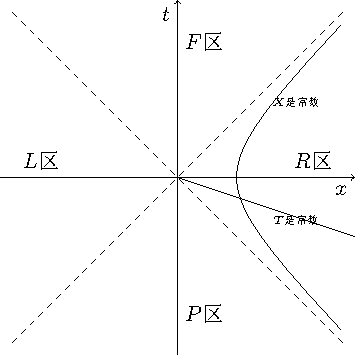
\includegraphics[width=5cm]{fig/II1-Rindler.pdf}
    \caption{Rindler坐标} \label{chsr:fig_Rindler}
\end{figure}


下面,我们仅以$R$区为例来讨论.
由式\eqref{chsr:eqn_Rindler-trans}易得
\begin{equation}\label{chsr:eqn_tx-TX}
    X^2= x^2-(ct)^2, \qquad \coth (\alpha T)= \frac{x}{ct} .
\end{equation}
我们也可将式\eqref{chsr:eqn_tx-sh-ch}中$\tau $变为$T$,$c^2 \alpha^{-1} $变为$X$;
同样可得到变换式\eqref{chsr:eqn_Rindler-trans}.
图\ref{chsr:fig_Rindler}中的双曲线表明:
不同的$X$值表示不同的火箭以不同的常加速度值在飞行.
$R$区式\eqref{chsr:eqn_Rindler-trans}的逆变换是:
\begin{equation}\label{chsr:eqn_Rindler-trans-inv}
    T=\frac{1}{\alpha} {\rm arcoth } \frac{x}{ct},\qquad
    X=\sqrt{x^2-(ct)^2} .
\end{equation}




直接计算可以得到$R$区非零的Christoffel记号是(下式中$T$是指$cT$)
\begin{equation}
    \Gamma^T_{TX}=\Gamma^T_{XT}=\frac{1}{X}, \qquad    \Gamma^X_{TT}=\frac{\alpha^2}{c^4} X .
\end{equation}
由此直接计算可得所有黎曼曲率的分量恒为零,
也就是Rindler度规\eqref{chsr:eqn_Rindler-megric}是
平直的,这说明Rindler时空本质上是闵氏时空.



下面我们来计算一下Rindler时空的共动观测者(定义见\S\ref{chfd:sec_comoving})的四加速度.
由\S\ref{chfd:sec_comoving}公式易知:
\begin{equation}
    Z^a =\frac{c^3}{X\alpha} \left(\frac{\partial}{\partial cT}\right)^a ;\qquad
    Z_a= -X\alpha  ({\rm d}T)_a .
\end{equation}
不难求得
\begin{equation}
    A^a = \nabla_Z Z^a = \frac{c^2}{X} \left(\frac{\partial}{\partial X}\right)^a .
\end{equation}
则有
\begin{equation}
    |A| = \sqrt{g_{ab} A^a A^b} = \frac{c^2}{X} .
\end{equation}
上面作了替换$c^2 \alpha^{-1} \to X$(见式\eqref{chsr:eqn_tx-TX}下面一行);
若反向执行则有$|A|=\alpha$.
这说明Rindler时空中共动观测者的四加速度模长是$\alpha$,
这与上一节给出的固有加速度相同.


由式\eqref{chsr:eqn_Rindler-trans}可得
\begin{equation}\label{chsr:eqn_dtx-dTX}
        \begin{pmatrix}
            {\rm d}ct \\ {\rm d}x
        \end{pmatrix}= 
        \begin{pmatrix}
          \frac{\alpha}{c^2} X\cosh \frac{\alpha}{c}T & \sinh\frac{\alpha}{c} T \\ 
          \frac{\alpha}{c^2} X\sinh \frac{\alpha}{c}T & \cosh\frac{\alpha}{c} T
        \end{pmatrix}
        \begin{pmatrix}
            {\rm d}cT \\ {\rm d}X
        \end{pmatrix}. 
\end{equation}
其逆变换是
\begin{equation}\label{chsr:eqn_dtx-dTX-inv}
\begin{pmatrix}
    {\rm d}cT \\ {\rm d}X
\end{pmatrix}= \frac{c^2}{\alpha X}
\begin{pmatrix}
    \cosh \frac{\alpha}{c}T & -\sinh \frac{\alpha}{c}T \\ 
 -\frac{\alpha}{c^2}X \sinh \frac{\alpha}{c}T & \frac{\alpha}{c^2}X \cosh \frac{\alpha}{c}T
\end{pmatrix}
\begin{pmatrix}
    {\rm d}ct \\ {\rm d}x
\end{pmatrix} .
\end{equation}
惯性系间的变换由洛伦兹变换描述.惯性系到匀加速运动参考系间的变换由式\eqref{chsr:eqn_Rindler-trans}、
\eqref{chsr:eqn_dtx-dTX}来描述;再结合式\eqref{chdm:eqn_tensor-component-trans}可以得到
两个参考系间张量的变换关系,比如电磁场张量$F_{\mu\nu}$.很明显经过式\eqref{chsr:eqn_dtx-dTX}变换
后的匀加速度参考系的麦克斯韦方程组与惯性系的麦氏方程组形式上不会相同.
如读者有兴趣可以试着推导一下Rindler坐标系下的麦氏方程组.




\begin{example}
	验证Rindler变换是等距的.
\end{example}
利用式\eqref{chdm:eqn_isometry-MMcoord}、\eqref{chsr:eqn_dtx-dTX},有
\setlength{\mathindent}{0em}
\begin{align*}
	\begin{pmatrix}
		\frac{\alpha}{c^2} X\cosh \frac{\alpha}{c}T & \sinh\frac{\alpha}{c} T \\ 
		\frac{\alpha}{c^2} X\sinh \frac{\alpha}{c}T & \cosh\frac{\alpha}{c} T
	\end{pmatrix}^T
	\begin{pmatrix}
		-1 & 0 \\ 0 & 1
	\end{pmatrix}
	\begin{pmatrix}
		\frac{\alpha}{c^2} X\cosh \frac{\alpha}{c}T & \sinh\frac{\alpha}{c} T \\ 
		\frac{\alpha}{c^2} X\sinh \frac{\alpha}{c}T & \cosh\frac{\alpha}{c} T
	\end{pmatrix} 
	=\begin{pmatrix}
		-\frac{\alpha ^2 X^2}{c^4} & 0 \\ 
		0 & 1
	\end{pmatrix} .
\end{align*}\setlength{\mathindent}{2em}
可见变换后的度规与式\eqref{chsr:eqn_Rindler-megric-RL}相同,故是等距变换.



\index[physwords]{麦克斯韦方程组}
\index[physwords]{电磁动力学}

\section{麦克斯韦方程组}\label{chsr:sec_maxwell}

\subsection{微分形式麦克斯韦方程组}
真空中麦克斯韦方程组(SI制)是
\begin{subequations}\label{chsr:eqn_maxwell-vac}
	\begin{align}
		\nabla \cdot  \boldsymbol{E} &= \dfrac{\rho }{\epsilon_0}, \label{chsr:eqn_gauss-e-vac} \\
		\nabla \cdot  \boldsymbol{B} &= 0,  \label{chsr:eqn_gauss-b-vac}\\
		\nabla \times \boldsymbol{E} +\frac{\partial \boldsymbol{B}}{\partial t} &= 0,  \label{chsr:eqn_faraday-vac}\\
		\nabla \times \boldsymbol{B} -\mu_0\epsilon_0\frac{\partial \boldsymbol{E}}{\partial t} &= \mu_0\boldsymbol{J}. \label{chsr:eqn_amp-max-vac}
	\end{align}
\end{subequations}
其中$\epsilon_0$是真空介电常数,$\mu_0$是真空磁导率常数;
$\boldsymbol{E}$是电场强度,$\boldsymbol{B}$是磁感应强度;
$\boldsymbol{J}$是自由电流密度矢量,$\rho$自由电荷密度.
\eqref{chsr:eqn_gauss-e-vac}是电场满足的库仑定律,也称为电场高斯定律.
\eqref{chsr:eqn_gauss-b-vac}是无自由磁单极子定律,偶尔有人称为磁场高斯定律.
\eqref{chsr:eqn_faraday-vac}是法拉第电磁感应定律.
\eqref{chsr:eqn_amp-max-vac}是安培-麦克斯韦定律.
这四个方程组合起来后构成了经典电磁场的第一基本假设,{\heiti 简称}为麦克斯韦方程组
{\footnote{正是这一“简称”,将本来属于法拉第、安培、库仑等电磁大师们的贡献
		{\heiti 有形}地转移到麦克斯韦头上.笔者不是说麦克斯韦不伟大,而是他被冠以本来属于法拉第、
		安培、库仑等大师的光环.麦克斯韦或许在数量上比法拉第、安培、库仑等大师伟大一些,但
		和这几个人的贡献没有量级上的差别.
		类似的简称还有非对易规范场中的Higgs机制.}}.
式\eqref{chsr:eqn_amp-max-vac}中的$\frac{\partial \boldsymbol{E}}{\partial t}$称为位移电流,
是麦克斯韦于1860年代引入的,这一项统一了电与磁;但此项并不是真正的电流.

电流电荷源满足电荷守恒定律,即
\begin{equation}\label{chsr:eqn_charge-conservation}
	\frac{\partial \rho}{\partial t} + \nabla \cdot \boldsymbol{J} = 0
	{\quad \color{red} \Leftrightarrow \quad }
	\frac{\partial J ^\mu}{\partial x^\mu} = 0; \quad
	\text{其中} \   J^\mu = (\rho c, \boldsymbol{J}).
\end{equation}

\index[physwords]{电荷守恒定律}

带电连续物质与电磁场间的相互作用是洛伦兹力密度矢量,
\begin{equation}\label{chsr:eqn_lorenz-force}
	\boldsymbol{f} = \rho \boldsymbol{E} + \boldsymbol{J}\times\boldsymbol{B}.
\end{equation}
它给出了单位体积电荷所受力密度矢量.
洛伦兹力的表达式是从实验中总结得到的,
这里面包含了库仑力、安培力.这是一个基本方程式,
好比两个天体间的引力是牛顿万有引力公式一样,
不能由其它理论推导得到.

麦克斯韦方程组\eqref{chsr:eqn_maxwell-vac}、电荷守恒定律\eqref{chsr:eqn_charge-conservation}和
洛伦兹力\eqref{chsr:eqn_lorenz-force}(再加上牛顿第二定律)构成了宏观电磁动力学
{\footnote{这门课程英文名称是Electro-Dynamics,直译过来就是{\fangsong 电动力学}.由于中英文的差异,
		{\kaishu 电动力学}经常被断句成{\kaishu 电动-力学}(包括笔者本人),然而正确的断句是
		{\kaishu 电-动力学};英文则没有这种断句错误.如果把它翻译成{\heiti 电磁动力学},则没有断句
		歧义,而且与此课程内容更为贴近.}}的基础,它们是相互独立的定律.

除了上述三个基本假设之外,笔者觉得还有一条隐含假设:
宏观电磁场可由两个矢量$\boldsymbol{E}$和$\boldsymbol{B}$完备描述.

%\subsection{含有磁荷的麦克斯韦方程组}
%前面的麦克斯韦方程组是不对称的,只有电流、电荷项,没有磁荷.
%补上磁荷后,有
%\begin{subequations}\label{chsr:eqn_maxwell-qm}
%    \begin{align}
	%        \nabla \cdot  \boldsymbol{E} &= \frac{\rho_e}{\epsilon_0}, \label{chsr:eqn_gauss-e-qm} \\
	%        \nabla \cdot  \boldsymbol{B} &= \mu_0 \rho_m,  \label{chsr:eqn_gauss-b-qm}\\
	%        \nabla \times \boldsymbol{E} +\frac{\partial \boldsymbol{B}}{\partial t} &= -\mu_0\boldsymbol{J}_m,  \label{chsr:eqn_faraday-qm}\\
	%        \nabla \times \boldsymbol{B} - \frac{1}{c^2}
	%        \frac{\partial \boldsymbol{E}}{\partial t} &= +\mu_0\boldsymbol{J}_e. \label{chsr:eqn_amp-max-qm}
	%    \end{align}
%\end{subequations}
%电荷、磁荷都是守恒的,有两个连续性方程
%\begin{subequations}\label{chsr:eqn_em-continuity}
%    \begin{align}
	%        \frac{\partial \rho_e}{\partial t} + \nabla \cdot \boldsymbol{J}_e &= 0 \label{chsr:eqn_e-continuity} \\
	%        \frac{\partial \rho_m}{\partial t} + \nabla \cdot \boldsymbol{J}_m &= 0 \label{chsr:eqn_m-continuity}
	%    \end{align}
%\end{subequations}
%洛伦兹力公式也需要推广,
%\begin{equation}\label{chsr:eqn_lorenz-force-em}
%    \boldsymbol{f} = \rho_e \boldsymbol{E} + \boldsymbol{J}_e\times\boldsymbol{B} \ + \
%    \rho_m \boldsymbol{B} - \boldsymbol{J}_m\times\boldsymbol{E}/c^2.
%\end{equation}
%截止到目前为止,实验上还没有发现自由磁单极子,所以有关磁单极子的
%理论都是数学,而非物理.
%
%如果做如下变量代换,方程式\eqref{chsr:eqn_maxwell-qm}形式不变,
%\begin{equation}\label{chsr:eqn_dual-em}
%    \begin{aligned}
	%        \boldsymbol{E}' &= \boldsymbol{E} \cos\theta + c\boldsymbol{B}\sin\theta, &
	%        c\boldsymbol{B}' &= c\boldsymbol{B}\cos\theta -\boldsymbol{E} \sin\theta, \\
	%        c \rho'_e &= c \rho_e\cos\theta + \rho_m\sin\theta, &
	%        \rho'_m &= \rho_m\cos\theta -c \rho_e\sin\theta, \\
	%        c \boldsymbol{J}'_e &= c \boldsymbol{J}_e\cos\theta + \boldsymbol{J}_m\sin\theta, &
	%        \boldsymbol{J}'_m &= \boldsymbol{J}_m\cos\theta -c \boldsymbol{J}_e\sin\theta.
	%    \end{aligned}
%\end{equation}
%其中$\theta$是一个与时空坐标、电磁场无关的任意实数,这个代换称为对偶变换.

\index[physwords]{电磁场张量}

\subsection{电磁张量形式麦克斯韦方程组}
与上节相似,我们只是罗列一些基本公式.
电磁场张量写成矩阵形式为
\begin{equation}
    F^{\mu\nu} = \begin{pmatrix}
        0 & E_x/c & E_y/c & E_z/c \\
        -E_x/c & 0 & B_z & -B_y \\
        -E_y/c & -B_z & 0 & B_x \\
        -E_z/c & B_y & -B_x & 0
    \end{pmatrix}.
\end{equation}
%可将它的指标进行升降,有
%\begin{align}
%    F_{\alpha}^{\cdot\nu}&= \eta_{\alpha\mu}F^{\mu\nu}
%    = \begin{pmatrix}
%        0 & -E_x/c & -E_y/c & -E_z/c \\
%        -E_x/c & 0 & B_z & -B_y \\
%        -E_y/c & -B_z & 0 & B_x \\
%        -E_z/c & B_y & -B_x & 0
%    \end{pmatrix}, \\
%    F^{\mu}_{\cdot\beta}&= F^{\mu\nu}\eta_{\nu\beta}
%    = \begin{pmatrix}
%        0 & E_x/c & E_y/c & E_z/c \\
%        E_x/c & 0 & B_z & -B_y \\
%        E_y/c & -B_z & 0 & B_x \\
%        E_z/c & B_y & -B_x & 0
%    \end{pmatrix}, \\
%    F_{\alpha\beta} &= \eta_{\alpha\mu}F^{\mu\nu}\eta_{\nu\beta}
%    = \begin{pmatrix}
%        0 & -E_x/c & -E_y/c & -E_z/c \\
%        E_x/c & 0 & B_z & -B_y \\
%        E_y/c & -B_z & 0 & B_x \\
%        E_z/c & B_y & -B_x & 0
%    \end{pmatrix}.
%\end{align}


四维协变形式的麦克斯韦方程组可以写成:
\begin{subequations}\label{chsr:eqn_maxwell-F}
    \begin{align}
        \partial_{\alpha} F^{\alpha\beta} &= -\mu_0 J^{\beta} ,   \label{chsr:eqn_maxwell-F1} \\
        \partial_\gamma F_{ \alpha \beta } + \partial_\alpha F_{ \beta \gamma }
        + \partial_\beta F_{ \gamma \alpha } &= 0. \label{chsr:eqn_maxwell-F2}
    \end{align}
\end{subequations}
\eqref{chsr:eqn_maxwell-F1}展开得\eqref{chsr:eqn_gauss-e-vac}和\eqref{chsr:eqn_amp-max-vac},
\eqref{chsr:eqn_maxwell-F2}展开得\eqref{chsr:eqn_gauss-b-vac}和\eqref{chsr:eqn_faraday-vac}.


\index[physwords]{电磁规范势} \index[physwords]{电磁矢量势} \index[physwords]{电磁标量势}

\subsection{规范势形式的麦克斯韦方程组}
真空中麦克斯韦方程组\eqref{chsr:eqn_maxwell-vac}
中的方程${\rm div} \boldsymbol{B}=0$表示没有自由磁单极子,
由矢量分析中知识可知存在矢量势$\boldsymbol{A}$满足
$\boldsymbol{B}=\nabla\times \boldsymbol{A}$;将此式带入法拉第定律
\eqref{chsr:eqn_faraday-vac}并交换时间、空间偏微商,就可以得到
$\nabla\times \boldsymbol{E} + \nabla\times \frac{\partial}{\partial t} \boldsymbol{A} = 0$;
进而可以得到
$ \boldsymbol{E} + \frac{\partial}{\partial t} \boldsymbol{A}  =- \nabla \phi$.
至此,我们得到如下变换式
\begin{subequations}\label{chsr:eqn_BE-poetential-gauge-trans}
	\begin{align}
		\boldsymbol{B} &= \nabla\times \boldsymbol{A},  \label{chsr:eqn_B-poetential-gauge-trans} \\
		\boldsymbol{E} &= -\frac{\partial}{\partial t} \boldsymbol{A}  - \nabla \phi .
		\label{chsr:eqn_E-poetential-gauge-trans}
	\end{align}
\end{subequations}
矢量势$\boldsymbol{A}$和标量势$\phi$统一在一起称为{\kaishu 规范势}函数.
需要注意,由于此时的电场是有旋的,所以这里的$\phi$和静电场中的电势不同.
将式\eqref{chsr:eqn_BE-poetential-gauge-trans}带入式\eqref{chsr:eqn_maxwell-vac}
并应用$c^2 \mu_0\epsilon_0=1$,就得到了规范势表示的麦克斯韦方程组
\begin{subequations}\label{chsr:eqn_maxwell-poetential}
	\begin{align}
		{\nabla ^2}\phi  + \frac{\partial}{\partial t} \nabla  \cdot \boldsymbol{A}
		&=  - \frac{\rho}{\epsilon _0}, \label{chsr:eqn_gauss-e-poetential} \\
		{\nabla ^2}\boldsymbol{A} - \frac{1}{c^2}\frac{\partial ^2\boldsymbol{A}}{\partial {t^2}}
		- \nabla \left( {\nabla  \cdot \boldsymbol{A} + \frac{1}{c^2}\frac{ \partial \phi }{ \partial t}} \right)
		&=  - {\mu _0}\boldsymbol{J}. \label{chsr:eqn_amp-max-poetential}
	\end{align}
\end{subequations}
其中\eqref{chsr:eqn_gauss-b-vac}和\eqref{chsr:eqn_faraday-vac}自动满足,
\eqref{chsr:eqn_gauss-b-vac}和\eqref{chsr:eqn_amp-max-vac}变成了上面两式.

因上面变换中没有指定矢量势$\boldsymbol{A}$的散度,
在如下变换下,方程\eqref{chsr:eqn_BE-poetential-gauge-trans}不变
\begin{subequations}\label{chsr:eqn_gauge-trans}
	\begin{align}
		\boldsymbol{A}' &= \boldsymbol{A} + \nabla f, \label{chsr:eqn_A-gauge-trans} \\
		\phi' &= \phi -\frac{\partial f}{\partial t} . \label{chsr:eqn_phi-gauge-trans}
	\end{align}
\end{subequations}
这个变换式叫做第一类{\heiti 规范变换}.带入后直接可验证
\begin{align*}
	\boldsymbol{B} &= \nabla\times \boldsymbol{A}' = \nabla\times \boldsymbol{A} + \cancel{\nabla \times\nabla f} , \\
	\boldsymbol{E} &= -\frac{\partial}{\partial t} \boldsymbol{A}'  - \nabla \phi' =
	-\frac{\partial}{\partial t} \boldsymbol{A}  \
	\cancel{- \frac{\partial \nabla f}{\partial t} }
	- \nabla \phi \
	\cancel{+ \nabla \frac{\partial f}{\partial t}}
	=-\frac{\partial}{\partial t} \boldsymbol{A}  - \nabla \phi .
\end{align*}
可见$(\phi,\boldsymbol{A})$和$(\phi',\boldsymbol{A}')$描述相同的电磁场$\boldsymbol{B},\boldsymbol{E}$.

规范变换\eqref{chsr:eqn_gauge-trans}可以写成四维协变形式,
\begin{equation}\label{chsr:eqn_gauge-trans-covariant}
	A^{\prime\mu} = A^\mu + \partial^\mu f; \qquad
	\text{其中} \  A^\mu \equiv (\phi/c,\boldsymbol{A}).
\end{equation}

我们可以把规范势和电磁张量关联起来了:
\begin{equation}\label{chsr:eqn_Fab}
    F^{\mu\nu} =\partial^\mu A^\nu - \partial^\nu A^\mu .
\end{equation}


\subsubsection{规范变换与边界条件}\label{chsr:sec_gauge-bc}
物理上只能给出$\boldsymbol{B}$的狄里克莱(第一类)边界条件,
这对应着矢量势一阶偏导数(第二类)边界条件,即
\begin{equation}
	\frac{\partial \boldsymbol{A}}{\partial n} = \boldsymbol{B} |_{\partial D},
	\quad \boldsymbol{B}|_{\partial D} {\text {表示区域$D$边界上的值,$n$是外法向.}}
\end{equation}
物理上无法给出矢量势$\boldsymbol{A}$在边界上的值(第一类或狄里克莱边条件),即
\begin{equation}
	\boldsymbol{A} |_{\partial D} = ?, \qquad \boldsymbol{A} {\text {在连通区域$D$边界上的值是未知的}.}
\end{equation}
如果我们把电磁场$\boldsymbol{B} $看作是已知的,
把\eqref{chsr:eqn_B-poetential-gauge-trans}看作是关于矢量势$\boldsymbol{A}$的方程,
即便配上后面所谓的规范条件(任意一种),那么方程组
\begin{equation}\label{chsr:eqn_A-poetential}
	\nabla\times \boldsymbol{A}  =\boldsymbol{B},\qquad \nabla\cdot \boldsymbol{A}  =\psi,
\end{equation}
由于$\boldsymbol{A}$只有一阶偏导数边界条件,物理上没有$\boldsymbol{A}$的
狄里克莱边条件,式\eqref{chsr:eqn_A-poetential}
的解也是无法唯一确定的
{\footnote{数学上,一阶偏微分方程组\eqref{chsr:eqn_A-poetential}需给定
		狄里克莱边界条件,不能给一阶偏微分边界条件.}}.
这就导致了即便给定规范条件(即补充了$\boldsymbol{A}$的散度方程),
仍旧存在规范变换\eqref{chsr:eqn_gauge-trans}.
这类在补充规范条件后,
由于无法给出$\boldsymbol{A}$狄里克莱边条件引起的规范变换叫作{\heiti 第二类规范变换}.
不论第一类还是第二类规范变换,它们的数学表达形式是相同的,
都为式\eqref{chsr:eqn_gauge-trans-covariant};也就是说
引起规范变换的原因有两个,一个是缺方程,一个是边界条件并能完全确定,
但它们具体变换的数学形式是相同的.

举个最简单的情形,我们令\eqref{chsr:eqn_A-poetential}中的$\boldsymbol{B}=0$、$\psi=0$,
那么\eqref{chsr:eqn_A-poetential}变成$\nabla\times \boldsymbol{A}  =0$、$ \nabla\cdot \boldsymbol{A}  =0$,
令$\boldsymbol{A}=\nabla\theta$,我们就可以把\eqref{chsr:eqn_A-poetential}变成$\nabla^2\theta=0$.
这是拉普拉斯方程,依照前面分析物理上只能给出$\partial^2\theta$边界条件,即$\theta$的
二阶偏导数边界条件.此方程解并不唯一.


\index[physwords]{规范条件}

\subsubsection{规范条件}
方程式\eqref{chsr:eqn_BE-poetential-gauge-trans}解不唯一,但它在
第\pageref{chmla:def_linear-dependence}页定义\ref{chmla:def_linear-dependence}下
是适定的;在定义\ref{chmla:def_diff-linear-dependence}下是欠定的.
依照定义\ref{chmla:def_diff-linear-dependence},
方程式\eqref{chsr:eqn_BE-poetential-gauge-trans}和
方程式\eqref{chsr:eqn_maxwell-poetential}都需要补充一个方程,
称之为{\kaishu 规范条件}.
由于物理上无法对规范条件提出明确要求,因此所补充的方程只要
能确保麦克斯韦方程组解的存在即可,不要求解的唯一性.但补充规范条件后,
需要方程变成较为简单的形式(或者你需要的形式),这可能是对规范条件唯一的要求.


%\subsubsection{库仑规范}
%库仑规范,也称为横场规范或者辐射规范,它是
%\begin{equation}\label{chsr:eqn_coulomb-gauge}
%    \nabla \cdot \boldsymbol{A} = 0.
%\end{equation}
%将上式带入\eqref{chsr:eqn_maxwell-poetential}后,可得
%\begin{subequations}\label{chsr:eqn_maxwell-poet-coul-gauge}
%    \begin{align}
	%        {\nabla ^2}\phi    &=  - \frac{\rho}{\epsilon _0}, \label{chsr:eqn_gauss-e-coul-gauge} \\
	%        {\nabla ^2}\boldsymbol{A} - \frac{1}{c^2}\frac{\partial ^2\boldsymbol{A}}{\partial {t^2}}
	%        - \frac{1}{c^2}\frac{ \partial \nabla\phi }{ \partial t}
	%        &=  - {\mu _0}\boldsymbol{J}. \label{chsr:eqn_amp-max-coul-gauge}
	%    \end{align}
%\end{subequations}
%这就是结合库仑规范的麦克斯韦方程组,需注意:
%\eqref{chsr:eqn_maxwell-poet-coul-gauge}一定要与规范\eqref{chsr:eqn_coulomb-gauge}
%结合在一起求解.之所以称之为库仑规范,是因为\eqref{chsr:eqn_gauss-e-coul-gauge}
%与静电场中的库仑定律在形式上完全一样;但需注意这里的$\phi${\heiti 不}是静电场的势函数.
%
%
%
%如果库仑规范不能满足,即$\Theta = \nabla \cdot \boldsymbol{A} \neq 0$,那么
%由\eqref{chsr:eqn_A-gauge-trans}知道可令新的矢势$\boldsymbol{A}'$满足库仑规范,即
%\begin{equation}
%    \nabla \cdot\boldsymbol{A}' = \nabla \cdot\boldsymbol{A} + \nabla^2 f {\color{red}\Rightarrow}
%    -\Theta =  \nabla^2 f .
%\end{equation}
%依照\S\ref{chsr:sec_gauge-bc}所述,对函数$f({x^\mu})$的边界条件没有什么限制,
%泊松方程$\nabla^2 f= -\Theta $解一定是存在的,也就是说库仑规范一定可以满足.
%新标量势可按照变换\eqref{chsr:eqn_phi-gauge-trans}来求取.
%
%
%
%对于库仑规范约束下,无界空间、无源、自由电磁场\eqref{chsr:eqn_gauss-e-coul-gauge}中的
%标量势可以恒为零,即$\phi =0$.需要注意,只是在满足诸多前提下,允许$\phi =0$的解存在,
%不能把$\phi =0$看成一条新的规范;规范条件只能补充一个,不能多于一个!

\index[physwords]{洛伦茨规范} \index[physwords]{Lorenz规范}

\subsubsection{洛伦茨规范}
丹麦物理学家洛伦茨{\footnote{L. V. Lorenz(洛伦茨)不是荷兰物理学家
		洛伦兹(H. A. Loren{\textcolor{red}{t}}z),
		他们俩的姓氏只差一个字母{\textcolor{red}{t}}.}}
于1867年提出如下方程
\begin{equation}\label{chsr:eqn_lorenz-gauge}
	{\nabla  \cdot \boldsymbol{A} + \frac{1}{c^2}\frac{ \partial \phi }{ \partial t}}  = 0,
\end{equation}
此方程被称为洛伦茨规范条件.将它带入
\eqref{chsr:eqn_maxwell-poetential}后,可得
\begin{subequations}\label{chsr:eqn_maxwell-lorenz-gauge}
	\begin{align}
		{\nabla ^2}\phi  - \frac{1}{c^2}\frac{\partial^2 \phi}{\partial t^2}
		&=  - \frac{\rho}{\epsilon _0}, \label{chsr:eqn_gauss-e-lorenz-gauge} \\
		{\nabla ^2}\boldsymbol{A} - \frac{1}{c^2}\frac{\partial ^2\boldsymbol{A}}{\partial {t^2}}
		&=  - {\mu _0}\boldsymbol{J}. \label{chsr:eqn_amp-max-lorenz-gauge}
	\end{align}
\end{subequations}
这就是结合洛伦茨规范的麦克斯韦方程组,同样需注意:
\eqref{chsr:eqn_maxwell-lorenz-gauge}一定要与规范\eqref{chsr:eqn_lorenz-gauge}
结合在一起求解.此时的方程式\eqref{chsr:eqn_maxwell-lorenz-gauge}是波动方程形式.


如果规范势$A_\mu$不满足洛伦茨规范,即$\Theta \equiv \partial_\mu A^\mu \neq 0$,
那么可作规范变换\eqref{chsr:eqn_gauge-trans-covariant}导致新的
规范势$A^{\prime}_{\mu}$满足洛伦茨规范:
\begin{equation}
	A^{\prime}_{\mu} = A_\mu + \partial_\mu f {\quad\color{red}\Rightarrow\quad}
	\partial^\mu A^{\prime}_{\mu} = \partial^\mu A_\mu + \partial^\mu\partial_\mu f
	{\quad\color{red}\Rightarrow\quad} \square f = - \Theta .
\end{equation}
依照\ref{chsr:sec_gauge-bc}节所述,对函数$f({x^\mu})$的边界条件没有多少限制,
那么上述波动方程$\square f = - \Theta$解是一定存在的,也就是说可以找到一个$f$使得
新的规范势$A^{\prime}_{\mu}$满足洛伦茨规范$\partial^\mu A^{\prime}_{\mu}=0$.
这也就说明了:我们一定有办法使洛伦茨规范得以满足.


\subsubsection{其它规范}
规范条件就是补充一个方程,有很多种\cite{jackson2002-LC},比如常用的库仑规范:
\begin{equation}
    \nabla \cdot \boldsymbol{A} = 0 .
\end{equation}
此外,再举一例
\begin{equation}\label{chsr:eqn_temporal-gauge}
	\phi = 0,
\end{equation}
它称为瞬时规范.
若原规范不满足规范\eqref{chsr:eqn_temporal-gauge},
即$\phi\neq 0$;
则由\eqref{chsr:eqn_phi-gauge-trans}可知
存在变换$\phi' = \phi -\frac{\partial f}{\partial t}$,
使新的$\phi' =0$,即
\begin{equation}
	\frac{\partial f}{\partial t} = \phi {\quad \color{red}\Rightarrow\quad}
	f(\boldsymbol{r},t) = \int^{t} \phi(\boldsymbol{r},\tau) {\rm d}\tau .
\end{equation}
这样,新的标势恒为零$\phi' =0$,新的矢势可由\eqref{chsr:eqn_A-gauge-trans}求得:
\begin{equation}
    \boldsymbol{A}' = \boldsymbol{A} + \nabla [ \int^{t} \phi(\boldsymbol{r},\tau) {\rm d}\tau ] .
\end{equation}




\subsubsection{规范势$A^\mu$是洛伦兹四矢量吗?}\label{chsr:sec_isAvec}
规范势$A^\mu =(\phi/c,\boldsymbol{A})$在不同规范下会有不同的形式,比如
在\eqref{chsr:eqn_temporal-gauge}式下,第零分量恒为零.这充分说明
在此规范下$A^\mu${\heiti 不}是四矢量.其原因是因为$A^\mu$是个物理量,
它存在规范自由度,可以取各种规范而不影响可观测物理结果.

在不指定规范条件的前提下,规范势$A^\mu$被{\heiti 人为地规定}为洛伦兹四矢量.
显然,如果选取的规范条件是洛伦兹协变的(比如洛伦茨规范条件),那么
规范势也是四矢量.
如果选取的规范条件{\heiti 不}是洛伦兹协变的(比如库仑规范或瞬时规范),
那么一般说来规范势{\heiti 不}是四矢量.










\index[physwords]{闵氏几何}

\section{四维闵氏几何语言讨论时空结构}\label{chsr:sec_spacetime-structure-Min}
前面几节仍旧采用1+3分量语言(时间和空间)来描述狭义相对论;
从本节开始,我们使用四维语言来从新描述.

我们已经知道在相对论中时间和空间已经不是绝对分离的了,两者有着密切关系.
闵可夫斯基曾经说过:从今以后,空间和时间本身注定要消失在完全的阴影之中,只有它们的某种结合才保持为独立的实体;
这就是闵氏几何.今天我们更加确信的是{\kaishu 时空}才是更为基本的物理概念,时间和空间
需要时空作1+3分解才能得到;先有时空,后有时间和空间;需注意时空不是简单的时间加空间.


为了简化问题,在本节我们采用自然单位制(见附录\ref{chunit-dim:sec_nature-units}),
即令$c=1$. %;但仍将$c$在公式中表出.

\subsection{引入流形}
在\S \ref{chsr:sec_srf}中,我们引入了“事件”这个概念;全部事件的集合称为{\heiti 时空}(Space-time);
从物理直觉上,我们可以假设“事件”充满整个时空,时空是一个四维连续系统
{\footnote{关于事件与时空关系的描述在很多书籍中都有,
比如\parencite[\S 3.2]{synge-1960}或\parencite[\S 3.1]{hawking-ellis1973}.
笔者没有查询到是哪位先贤最早认识到此点,我猜测可能是闵可夫斯基或者爱因斯坦.}}.
我们在这个四维连续系统上建立一个坐标系$\{x^\mu\}$,从狭义相对论基本原理出发,已经得到在
任意坐标变换下($x^\mu \to x^{\prime \mu}$)“间隔”$s^2$是一个不变量,这说明间隔是
脱离某套具体坐标系的,或者说间隔是与坐标系无关的物理量.

数学上“微分流形”虽然也是建立在具体(局部)坐标上的,但个坐标间必须相互容许,
所以流形也是不依赖于某套具体坐标的.这与“时空”中间隔$s^2$的属性基本相同.
既然有这种相似性,我们可以借用数学上“微分流形”这一概念来描述物理上的“时空”.
物理上用四个实参数来描述事件,我们自然用数学上的四维光滑流形来描述物理上的时空.

%从“元间隔”\eqref{chsr:eqn_interval-inv-ds}可以看到并非所有项都是“正的”,有一项前的系数是“负的”.
很容易从闵氏时空的弧长公式\eqref{chrg:eqn_arc-length}看出来其元长度是
\begin{equation}
    {\rm d}s^2 = -({\rm d}x^0)^2 +({\rm d}x^1)^2 +({\rm d}x^2)^2 +({\rm d}x^3)^2 .
\end{equation}
这与狭义相对论中得到“元间隔”\eqref{chsr:eqn_interval-inv-ds}完全吻合;
因此狭义相对论时空对应的流形正是我们之前定义的四维平直
闵可夫斯基时空\ref{chdm:def_MinkowskiSpace}或定义\ref{chrg:def_Minkowski-space}.

我们大致按照狭义相对论发展的历史顺序,将“事件”与“流形”挂钩,然后再将“正定”度规拓展到“不定”度规(这
是闵可夫斯基的重大发现).有了这样的认识之后,才将“闵氏度规”推广到纯数学的流形论中;
在此之前,纯数学几乎只研究正定度规情形.
先有物理上的狭义相对论,数学中微分几何才诞生“闵氏空间”这一概念.


现今的物理学已经搞清楚:{\bfseries (1)} 狭义相对论的背景时空是四维平直空间(黎曼曲率为零);
{\bfseries (2)} 它的度规类型是洛伦兹的,即度规特征值是$(-1,1,1,1)$.




\subsection{1+3分解}\label{chsr:sec_1+3decom}
现在看一下,我们手头有哪些东西.首先,有四维平直闵氏时空;
其次,知道在时空中“间隔”是不变的,不论你选择哪套坐标系,间隔都是同一数值.

至此,还没有时间、空间概念;只有四维平直时空和间隔不变性.

由\S\ref{chrg:sec_local-EuclideanSpace}知识可知,四维\CJKunderwave{平直空间}中存在局部
坐标系$(x^0,x^1, x^2, x^3)$使得度规在此坐标系下为$\eta={\rm diag}(-1,1,1,1)$,
即此坐标系是正交归一的.平直空间是可以用一个坐标域覆盖住的,
故我们可以把平直闵氏时空记为:$(\mathbb{R}^4_1,\eta)$.
我们把对应度规中$-1$那个坐标$x^0$称为“时间”,其它三个坐标$(x^1, x^2, x^3)$构成的子流形称为“空间”.
如果换另外一套坐标$(x^{\prime 0},x^{\prime 1}, x^{\prime 2}, x^{\prime 3})$来
描述$\mathbb{R}^4_1$,根据“间隔”不变性可知从$x^\mu$到$x^{\prime \mu}$的变换
一定是洛伦兹变换\eqref{chsr:eqn_lorentz-transofrm-x}或其逆变换;
变完之后的坐标$x^{\prime 0}$仍称为“时间”,其它三个坐标称为“空间”.


下面我们给出两个例子,它们不显示表出时间.

第一个例子.狭义相对论中的闵氏时空是平直的,它的切空间就是自身.
洛伦兹度规在坐标系$\{x^\mu\}$中可表示为
\begin{equation}\label{chsr:eqn_Lorentz-metric}
	\eta_{ab} = -({\rm d}x^0)_a ({\rm d}x^0)_b+({\rm d}x^1)_a({\rm d}x^1)_b
	+({\rm d}x^2)_a ({\rm d}x^2)_b+({\rm d}x^3)_a({\rm d}x^3)_b .
\end{equation}
在四维平直闵氏时空中,并不是任意一套坐标系都能显示表述“时间”.比如令
\begin{equation}
	u= x^0 - x^3, \qquad v= x^0 + x^3.
\end{equation}
此时度规\eqref{chsr:eqn_Lorentz-metric}变为
\begin{equation}\label{chsr:eqn_Lorentz-metric-light}
	\eta_{ab} = -\frac{1}{2}({\rm d}v)_a ({\rm d}u)_b
	-\frac{1}{2}({\rm d}u)_a ({\rm d}v)_b
	+({\rm d}x^1)_a({\rm d}x^1)_b +({\rm d}x^2)_a ({\rm d}x^2)_b.
\end{equation}
很容易看到新坐标$u,v$都是类光的;
那么从表面上来看,新的坐标系$\{u,v,x^1,x^2\}$没有显示“时间”的概念;
而是隐藏在$\{u,v\}$之中.

第二个例子.在闵氏时空中,甚至所有坐标基矢都可以是类空的.我们以二维时空为例,设有
$\eta_{ab} = -({\rm d}t)_a ({\rm d}t)_b+({\rm d}x)_a({\rm d}x)_b$,作变换
\begin{equation*}
	4u= 2t + x, \quad 4v= 2t-x
	\quad \Leftrightarrow \quad
	t= u+v,\quad x= 2(u-v).
\end{equation*}
我们不难求得新坐标$\{u,v\}$的时空属性
\begin{align*}
	\eta_{ab} \left(\frac{\partial}{\partial u}\right)^a \left(\frac{\partial}{\partial u}\right)^b 
%	=&\eta_{ab} \left[\left(\frac{\partial}{\partial t}\right)^a \frac{\partial t}{\partial u} +
%	\left(\frac{\partial}{\partial x}\right)^a \frac{\partial x}{\partial u} \right]
%	\left[\left(\frac{\partial}{\partial t}\right)^b \frac{\partial t}{\partial u} +
%	\left(\frac{\partial}{\partial x}\right)^b \frac{\partial x}{\partial u} \right] \\
	=& -\left(\frac{\partial t}{\partial u}\right)^2 +	\left( \frac{\partial x}{\partial u}\right)^2
	= -1 + (+2)^2 =3. \\
	\eta_{ab} \left(\frac{\partial}{\partial v}\right)^a \left(\frac{\partial}{\partial v}\right)^b 
%	=&\eta_{ab} \left[\left(\frac{\partial}{\partial t}\right)^a \frac{\partial t}{\partial v} +
%	\left(\frac{\partial}{\partial x}\right)^a \frac{\partial x}{\partial v} \right]
%	\left[\left(\frac{\partial}{\partial t}\right)^b \frac{\partial t}{\partial v} +
%	\left(\frac{\partial}{\partial x}\right)^b \frac{\partial x}{\partial v} \right] \\
	=& -\left(\frac{\partial t}{\partial v}\right)^2 +	\left( \frac{\partial x}{\partial v}\right)^2
	= -1 + (-2)^2 =3. 
\end{align*}
由上式可见新坐标$\{u,v\}$是类空的,不显含时间.


\subsection{时空图}\label{chsr:sec_spacetime}
我们先介绍四维{\heiti 时空图}:取纵坐标为$t\equiv x^0$代表时间;横坐标$x$代表三维空间,
但平面图上无法画出,所以压缩成一维;见图\ref{chsr:pic_spacetime}所示.平面图上
可以画出立体图,此时可以考虑两维空间方向,但仍必须压缩掉一维空间.
\begin{figure}[htb]
    \centering
    \begin{tikzpicture}[scale=3]
    \fill[lightgray] (0,0) -- (0.8,0.8)-- (-0.8,0.8)-- (0,0);
    \fill[lightgray] (0,0) -- (-0.8,-0.8)-- (0.8,-0.8)-- (0,0);
    \draw [-latex] (-1,0)--(1,0) node[above ] { $x$};
    \draw [-latex] (0,-1)--(0,1) node[right ] {$t$};
    \draw [-]  (-0.8,-0.8)node[below] {$P$}--(+0.8,0.8) node[above ] {$F$};
    \draw [-]  (+0.8,-0.8)node[below] {$P$}--(-0.8,0.8) node[above ] {$F$};
    \node at (-0.2,-0.1)  {$O$};
    \node at (-0.1,+0.4) {I};
    \node at (0.1,-0.3) {II};
    \node at (-0.5,0.1) {III};\node at (+0.5,0.1) {III};
    \draw [color=red](-0.6,-0.9) .. controls (-0.3,-0.7)and (-0.1,-0.2) .. (0,0);
    \draw [color=red](0,0) .. controls (0.1,0.2)and (0.3,0.7) .. (0.6,0.9);
%    \draw [color=green](-0.2,0.0)--(-0.2,0.9);
    \draw [color=blue] (0,0)--(0.3,0.9);
    \end{tikzpicture}
    \caption{质点世界线,时空分类}\label{chsr:pic_spacetime}
\end{figure}

前面介绍过的事件概念就是时空图中的一个点,全部点的集合就是闵氏时空.在狭义相对论范畴内,
我们仍需假设时空是四维连续的、连通的空间,这个空间的度规是洛伦兹度规.
质点(包括有质量和无质量的粒子)在时空中运动(包括静止不动情形),对应为时空图上一条曲线,称为该质点
的{\heiti 世界线},它能代表质点的全部历史;例如见图\ref{chsr:pic_spacetime}中红色曲线.
我们看一些具体问题.

\begin{example}
    一个静止不动的质点在时空图里的世界线是什么样的?
\end{example}
这个答案很容易想到,质点静止不动,就是在空间上没动,那么它的$x$坐标一直不变,
但是时间依然在流逝,也就是它的时间坐标在一直变大.所以,静止不动质点的世界线是一条跟$t$轴平行,
垂直于$x$轴的直线;例如图\ref{chsr:pic_spacetime}中$t$轴本身就是某质点世界线,
此质点位于三维空间坐标原点.
\qed

\begin{example}
一个匀速运动的粒子的世界线是什么样的?
\end{example}
速度的定义依旧是$\boldsymbol{u}={\rm d}\boldsymbol{x}/{{\rm d}t}$,匀速运动意味着$x=u t$;
那么这个质点的世界线应该是一条斜直线;如图\ref{chsr:pic_spacetime}中的
蓝色线,斜率的倒数就是其速度,即$t=1/u x$.
由此易得:{\kaishu 世界线的切线斜率就是该质点在此处的速度的倒数}.
\qed

\begin{example}
一条朝右上方$45^{\circ}$的斜直线,也就是图\ref{chsr:pic_spacetime}中的$OF$代表什么世界线?
\end{example}
$45^{\circ}$的斜直线的斜率就是1,因已约定光速$c=1$,故它代表光子世界线.
光子世界线实际上这是一个旋转超曲面,所以左上方也标记为$F$(future);而下方标记为$P$(past).
\qed

从这里我们可以看到,在时空图里,光子的世界线是$45^{\circ}$的斜直线.
我们也知道在相对论里任何有质量粒子的速度都是小于光速的,
那么一个有质量粒子的世界线该是什么样呢?是在区域I还是区域II或者区域III?
为了简单起见我们只分析从原点出发的质点运动.
我们可以这样想一下:如果粒子的速度比光速小,那么它的世界线切线斜率倒数就应该小于1,
也就是更靠近$t$轴;
%{\footnote{注意速度是距离除以时间,所以小于1是指更靠近时间轴,不是靠近空间轴$x$.}}
因此速度在静止和光速之间的质点世界线切线斜率倒数自然就是在区域I或II中了;
比如图中的红色曲线、蓝色斜直线.如果世界线切线斜率倒数大于1,
也就是位于III区中,“速度”是超光速的,自然界不存在这样的粒子.


\subsection{时空分类}\label{chsr:sec_stc}
时空中有两个事件$O$和$Q$,将$O$取为时空图的原点.
时空间隔是参考系变换的不变量,也就是洛伦兹变换下的不变量.根据时空间隔\eqref{chsr:eqn_interval-inv-ds},
即${\rm d}s^2 = -{\rm d}t^2 +{\rm d}x^2 +{\rm d}y^2 +{\rm d}z^2 =-{\rm d}t^2 (1-u^2)$,
物理学中约定:

\noindent\fbox{甲} 当${\rm d}s^2 <0 $时,时空为{\heiti 类时},
见图\ref{chsr:pic_spacetime}中I区和II区,已标记为阴影区.当$Q$点位于I区时,
直线$OQ$斜率倒数小于1,说明它的速度是亚光速的,并且从$O$点走到$Q$的过程中,时间$t$一直
是增加的;I区称为绝对未来.当$Q$点位于II区时,直线$OQ$斜率倒数小于1,说明它的速度是亚光速的;
但是从$O$点走到$Q$的过程中,时间$t$一直是减少的;II区称为绝对过去.
由于连续洛伦兹变换不改变
时间的正负,所以区域I和II是不可能通过洛伦兹变换相联系的;这种划分是绝对的.
有质量粒子世界线必须是类时的,指其切线斜率倒数小于1,即其速度为亚光速.


\noindent\fbox{乙} 当${\rm d}s^2 =0 $时,时空为{\heiti 类光},
见图\ref{chsr:pic_spacetime}中$OF,OP$斜率为1的直线,其实
为旋转超曲面,只不过在这张图中显示为直线.这个超曲面上的事件皆可由光联系.
其中$OF$指向绝对未来,$OP$指向绝对过去.
无质量粒子世界线必须类光.

\noindent\fbox{丙} 当${\rm d}s^2 >0 $时,时空为{\heiti 类空},
见图\ref{chsr:pic_spacetime}中III区,已标记为空白区.当$Q$点处于这一区域时,
直线$OQ$斜率倒数大于1,说明它的“速度”是超光速的,不对应自然界中任何粒子或物质.这个
区域的任何两个事件没有因果关系,可以通过洛伦兹变换改变事件的发生时序.
如果选择两参考系速度差$v$的范围是$c^2\frac{\Delta t}{\Delta x}<v<c$,
那么就可以颠倒事件$O$和$Q$的先后顺序;但
这不违反因果律,因为这两个事件没有因果关系.

在第\ref{chsr:sec_lorentz-transofrm}节末尾曾经讨论过洛伦兹变换把光速变成光速,
把亚光速变成亚光速,把超光速变成超光速;所以在洛伦兹变换下上述划分是绝对的,
变换前后不会出现跨区现象.

物理上,我们有间隔不变性,上面根据它把四维闵氏时空作了分类.
这种分类自然与定义\ref{chrg:def_vector-property}相互自洽;
因为历史上,我们先有间隔不变性,作了上述时空分类,然后
把这种分类方式推广到一般的流形中去的.

有了上述分类,我们称类时和类光矢量为{\heiti 因果矢量}.

在本节中,我们没有把数学上的定义\ref{chrg:def_vector-property}直接拿过来使用,
而是从物理角度再次给出定义;两者当然是相同的.
这样做的目的,是想更物理一些,不想让数学掩盖物理.


\subsection{固有时与坐标时}\label{chsr:sec_proper-time}
我们以图\ref{chsr:pic_spacetime}中红色类时世界线为例,此线所在的$t-x$系为惯性系$S$,称为静系或实验室系;
这条曲线上某个确定点$p$的时空坐标第0分量称为该点在$S$系的{\heiti 坐标时}.
也就是任意一质点在时空中运动时,建立某参考系及坐标系后,它的世界线上的类时坐标就是它的坐标时.

这条红色类时线的质点可能不是在作惯性运动.它在某时空点的3-速度是$\boldsymbol{u}$,我们就建立一个相对$S$系
以$\boldsymbol{u}$运动的临时惯性系$S'_u$;以$\boldsymbol{u}$运动的质点相对于$S'_u$系是静止的;我们称$S'_u$为
{\heiti 瞬时惯性系}.\index[physwords]{瞬时惯性系}
在下一临近时刻此质点的3-速度是$\boldsymbol{u}+{\rm d}\boldsymbol{u}$,我们再建立一个相对$S$系
以$\boldsymbol{u}+{\rm d}\boldsymbol{u}$运动的惯性系$S'_{u+{\rm d}u}$,此时的质点相对于$S'_{u+{\rm d}u}$系也是静止的.
我们可以在它世界线的每一点都建立一个这样的瞬时惯性系.




%在\ref{chsr:sec_time-dilation}节,
我们将{\heiti 固有时}定义为:一个相对参考系静止的时钟所记录的时间.
我们在这个时钟的类时世界线上每一点都建立一个瞬时惯性系,那么此时钟就相对
这个瞬时惯性系静止,它记录的时间就是{\heiti 固有时}.
既然相对瞬时惯性系静止,那么无穷小固有时${\rm d}\tau$正比于此时钟在这个
瞬时惯性系的无穷小时空间隔,它们的关系是${\rm d}s^2=-c^2{\rm d}\tau^2$.
${\rm d}s$就是世界线的的线元长度,
那么固有时也就是正比于世界线的线长,关系是
\begin{equation}
\tau = \frac{1}{c}\int \sqrt{-{\rm d}s^2},
\qquad \text{显示写出了光速}c .
\end{equation}
我们知道任意类时线的元线长是
${\rm d}s^2=-{\rm d}t^2 + {\rm d}x^2+{\rm d}y^2+{\rm d}z^2=-(1-u^2){\rm d}t^2$,结合
固有时即世界线线长的几何意义后有
\begin{equation}
{\rm d}\tau =\sqrt{-{\rm d}s^2}={\rm d}t \sqrt{1-u^2} \equiv \gamma_u^{-1}{\rm d}t,
\quad \gamma_u^{-1}= \sqrt{1-u^2}.
\end{equation}
其中${\rm d}t$是$S$系坐标时.
注意这里的$\gamma_u$与洛伦兹变换\eqref{chsr:eqn_lorentz-transofrm-x}中
$\gamma$不同,那里的速度$v$是两个惯性系速度差,这里的$u$是质点自身速率,
是质点所处瞬时惯性系与$S$系的速度差.
如果质点世界线是一条闵氏直线,其速度$u$是一个常数$v$.
如果质点速度$u=0$,那显然它的坐标时就是固有时.

{\kaishu 因固有时几何意义就是类时世界线线长,所以脱离世界线固有时无定义.}

当世界线为类光时,线长恒为零,所以光子世界线的固有时恒为零;
这说明光子上时间是凝固的.
除此以外还有光子四速度趋于无穷大.
以上几点都说明:光子不能充当参考系,任何
以光子为参考系的描述中必然会出现各种无穷大.





\subsection{闵氏曲线}
在平直闵氏时空中,无需使用微分几何工具(比如弧长变分)就能解决很多问题.
平直时空基矢场$(\frac{\partial }{\partial x^\mu})^a$和$({\rm d}x^\mu)_a$是
常矢量,我们将省略不写出,而使用分量语言讨论问题.

我们看一下动系的时空坐标是什么样子.
洛伦兹变换\eqref{chsr:eqn_lorentz-transofrm-x}是
$t' = \gamma ({t-v x})$,$  x' = \gamma ({x-vt})$.
在静系$t-x$中,$t'$轴就是$x'=0$的世界线,也就是原点$O'$的世界线,必然类时;由洛伦兹变换容易得到
它在$t-x$系的方程是$x=vt$,就是斜率倒数是速度$v$的过原点斜直线.
在静系$t-x$中,$x'$轴就是$t'=0$的世界线,必然类空;由洛伦兹变换容易得到
它在$t-x$系的方程是$t=vx$,就是斜率是$v$的过原点斜直线.如图\ref{chsr:pic_st1}左图所示红色轴就是动系坐标轴;
蓝色点划线是光子世界线.

虽然在图中红色线貌似不正交,这是在用欧氏观点来看;在闵氏几何下$t'$和$x'$线是正交的.
先看静系坐标轴自身的正交情况.静系$t$轴的切线方向在静系坐标是$(1,0,0,0)$
{\footnote{因$t$轴$x$轴等是直线,其切线方向处处相同,就是坐标轴指向方向.}},
静系$x$轴的切线方向在静系坐标是$(0,1,0,0)$;闵氏内积为
$(1,0,0,0) \eta  (0,1,0,0)^{T}=0$;说明两轴正交.
动系$t'$轴的切线方向在静系坐标是$(1,v,0,0)$,
动系$x'$轴的切线方向在静系坐标是$(v,1,0,0)$;
依闵氏几何(注意洛伦兹度规)有
$(1,v,0,0) \eta(v,1,0,0)^{T}=({\color{red}{\mathbf{-}}}1,v,0,0)\cdot(v,1,0,0)^{T}=0$;
这就证明了图\ref{chsr:pic_st1}左图中红色动系时间轴和空间轴是闵氏正交的.
读者需谨慎注意欧氏与闵氏空间的这种差别.图\ref{chsr:pic_st1}右图将动系画成了
正交形式,静系貌似不正交,其实是闵氏正交的,请读者验证右图正交性.
依照前面给出的新系在旧系的坐标不难论证$t$和$t'$轴夹角$\theta$等于$x$和$x'$夹角,
新旧两系的时间轴和空间轴各自都沿光子世界线对称.
左右两幅图是等价的.

\begin{figure}[htb]
    \centering
    \begin{tikzpicture}[scale=3]
%    \fill[lightgray] (0,0) -- (0.8,0.8)-- (-0.8,0.8)-- (0,0);
    \draw [-latex] (0,0)--(1,0) node[right ] {$x$};
    \draw [-latex] (0,0)--(0,1) node[left ]  {$t$};
    \draw [dash dot, blue]  (0,0)--(0.9,0.9); %node[above ] {光子世界线};
    \draw [red,-latex] (0,0)--(1,0.2) node[right ] {$x'$};
    \draw [red,-latex] (0,0)--(0.2,1) node[right ] {$t'$};
    \node at (0.5,0.05) {$\theta$};
    \node at (0.05,0.5) {$\theta$};
    \end{tikzpicture} \qquad
    \begin{tikzpicture}[scale=3]
    \draw [red,-latex] (0,0)--(1,0) node[right ] {$x'$};
    \draw [red,-latex] (0,0)--(0,1) node[right ] {$t'$};
    \draw [dash dot, blue]  (0,0)--(0.9,0.9); %node[above ] {光子世界线};
    \draw [-latex] (0,0)--(1,-0.2) node[right ] {$x$};
    \draw [-latex] (0,0)--(-0.2,1) node[right ] {$t$};
    \node at (0.5,-0.05) {$\theta$};
    \node at (-0.05,0.5) {$\theta$};
    \end{tikzpicture}
    \caption{不同惯性系时空图}\label{chsr:pic_st1}
\end{figure}

我们用图\ref{chsr:pic_st1}再来解释一下时空的“1+3”分解.
$\{t,x\}$是一种“1+3”分解,$\{t',x'\}$也是一种“1+3”分解,
可见这种分解方式有无穷多种.在时空图上来看,“1+3”分解无非是
先选出一个类时矢量场的参数$t$,依据它可以将时空分层为不相交的类空超曲面.
不同“1+3”分解分出来的时间$t$和$t'$自然不会相同,
这也就是为何相对论中会有很多套时间和空间的原因.
不同的“1+3”分解就意味着选择了不同的参考系.

闵氏空间与欧氏空间的差别不仅体现在正交性上,在曲线长度上也有区别.
式\eqref{chrg:eqn_arc-length}给出一般闵氏曲线长度定义,当曲线是直线时,其长度
就是时空间隔的绝对值.设点$p$时空坐标是$(t,x)$,$op$为连接原点$o$与点$p$的直线段,
见图\ref{chsr:pic_st2};其闵氏线长为$l_{op}=\sqrt{|-t^2+x^2|}$,可见双曲线
$s^2\equiv -t^2+x^2={\text{\kaishu 常数}}$上各点与原点$o$所连直线段等长;
例如$l_{oa}=l_{op}$,但按欧氏度规显然这两段直线不等长;画时空图时需时刻注意闵氏几何.
图\ref{chsr:pic_st2}中的双曲线称为{\heiti 校准曲线},它可以位于空间轴,也可以位于时间轴上.
比如位于时间轴上的双曲线上两点$b,q$,$l_{ob}$自然等长于$l_{oq}$.

时空中有任意可由类时线联系的两点$o$和$b$,此两点间最长的线是闵氏直线$ob$,其它任何闵氏非直线线长都
小于直线线长.前面我们已说明任何类时闵氏直线都可以当成一个新时间轴$t$,然后时空可以向
这个新系作1+3分解;为简单起见选$o$点当原点,即$t=0$,闵氏直线$oab$如图\ref{chsr:pic_line}所示.
另有连接$o$和$b$的类时红色曲线$ocb$.我们用许多垂直于$t$轴的蓝色直线将$ob$和$ocb$分成很多元线段,
这些元线段都是无穷小量;我们取$a$点坐标是$(x_0,0)$,$c$点坐标是$(x_0,x_1)$.
则线元$oa$和$oc$的闵氏长度是
$l_{oa}=\sqrt{|-(x_0)^2+(0)^2|}=x_0$,$l_{oc}=\sqrt{|-(x_0)^2+(x_1)^2|}$,因$oc$是类时线($|x_1|<|x_0|$),所以
有$l_{oa} > l_{oc}$;即每段元线段比较后都有直线段最长,所以直线段$l_{oab}$长于曲线段$l_{ocb}$.

\begin{figure}[htb]
    \begin{minipage}[t]{0.3\textwidth}
    \centering
    \begin{tikzpicture}[scale=3]
    %    \fill[lightgray] (0,0) -- (0.8,0.8)-- (-0.8,0.8)-- (0,0);
    \draw [-latex] (-0.6,0)--(0.7,0) node[right ] {$x$};
    \draw [-latex] (0,-0.5)--(0,0.7) node[left ]  {$t$};
    \draw [dash dot, blue]  (0,0)--(0.6,0.6); %node[above ] {光子世界线};
    \def\ax{0.3} ;    \def\by{0.3} ;
    \draw[domain=-58:60] plot ({\ax*sec(\x)},{\by*tan(\x)});
    \draw[domain=-60:60] plot ({\by*tan(\x)},{\ax*sec(\x)});
    \draw [-] (0,0) node[below left] {$o$} -- ({\ax*sec(-40)},{\by*tan(-40)}) node[right] {$p$};
    \filldraw ({\ax*sec(-40)},{\by*tan(-40)}) circle[radius=0.4pt];
    \filldraw ({\ax*sec(0)},{\by*tan(0)}) node[above right] {$a$} circle[radius=0.4pt];
    \draw [-] (0,0) -- ({\ax*tan(-40)},{\by*sec(-40)}) node[right] {$q$};
    \filldraw ({\ax*tan(-40)},{\by*sec(-40)}) circle[radius=0.4pt];
    \filldraw ({\ax*tan(0)},{\by*sec(0)}) node[above right] {$b$} circle[radius=0.4pt];
    \end{tikzpicture}
    \caption{校准曲线}\label{chsr:pic_st2}
    \end{minipage}
    \begin{minipage}[t]{0.3\textwidth}
    \centering
    \begin{tikzpicture}[scale=3.2]
    \draw [-latex] (0,0)node[below] {$o$} --(0,0.8)node[right] {$b$}--(0,1) node[left]  {$t$};
    \draw [-,red](0,0) .. controls (0.1,0.3)and (0.08,0.6) .. (0,0.8);
    \draw [-,blue](0,0.3)node[left] {$a$}--(0.065,0.3)node[right] {$c$};
    \draw [-,blue](0.0,0.6)--(0.056,0.6);
    \draw [-,blue](0.0,0.45)--(0.07,0.45);
    \filldraw (0,0.0) circle[radius=0.4pt]; % o
    \filldraw (0,0.3) circle[radius=0.2pt]; % a
    \filldraw (0.065,0.3) circle[radius=0.2pt]; % c
    \filldraw (0,0.8) circle[radius=0.4pt]; % b
    \end{tikzpicture}
    \caption{直线最长}\label{chsr:pic_line}
    \end{minipage}
    \begin{minipage}[t]{0.35\textwidth}
    \centering
    \begin{tikzpicture}[scale=3.5]
    %    \fill[lightgray] (0,0) -- (0.8,0.8)-- (-0.8,0.8)-- (0,0);
    \draw [-latex] (-0.3,0)--(1,0) node[right ] {$x$};
    \draw [-latex] (0,0)--(0,1) node[left ]  {$t$};
%    \draw [dash dot, blue]  (0,0)--(0.9,0.9); %node[above ] {光子世界线};
    \draw [red,-latex] (0,0)--(1,0.3) node[right ] {$x'$};
    \draw [red,-latex] (0,0)--(0.3,1) node[right ] {$t'$};
    \draw [dashed] (-0.2,0.5)--(0.7,0.5) node[right,font=\scriptsize] {$t=t_0$};
    \draw [dashed,red] (-0.2,0.34)--(0.7,0.61) node[right,font=\scriptsize] {$t'=t'_0$};
    \end{tikzpicture}
    \caption{同时的相对性}\label{chsr:pic_relativity-of-simultaneity}
    \end{minipage}
\end{figure}

\begin{example}
    孪生女佯谬.\index[physwords]{孪生女佯谬}
    地球上有一对孪生姐妹,姐姐名{\fangsong 花}妹妹名{\fangsong 红}.
    姐姐{\fangsong 花}坐宇宙飞船去旅行,妹妹{\fangsong 红}留在地球.若干年后姐姐{\fangsong 花}返回
    地球,问:此时两人年龄孰大孰小?
\end{example}
利用图\ref{chsr:pic_line}可以定性解释孪生子女佯谬.
既然姐姐{\fangsong 花}从地球出发再次返回地球,那她的旅程一定是类时世界线,
并且这条类时线的4-加速度不是零,也就是姐姐{\fangsong 花}不可能
一直作匀速直线运动,否则飞船是不可能再次返回地球的;
可以用图\ref{chsr:pic_line}的$ocb$表示.$o$表示当初两姐妹分别时刻,
$b$表示若干年后两姐妹再次相遇时刻.地球可以近似看成惯性系,直线$oab$可代表
处在地球上的妹妹{\fangsong 红}的世界线.上面我们说了固有时即线长,且$l_{oab}>l_{ocb}$,那么
也就是说处在地球上的妹妹{\fangsong 红}年纪大,坐飞船旅行姐姐{\fangsong 花}年纪小;
从而姐姐变妹妹,妹妹变姐姐.这种年龄上的改变是绝对的,不是相对的,原因是
飞船从地球出发再次返回地球,它不可能做匀速运动,肯定有洛伦兹四加速度.
\qed

\subsection{同时的相对性}
经过前面几小节的准备,我们现在用闵氏几何的方式来讨论同时相对性、钟缓尺缩等问题;
闵氏几何方法是将四维不变量作1+3分解后来研究这些问题的.
本小节内容可见图\ref{chsr:pic_relativity-of-simultaneity},
图中黑色坐标系$t-x$代表静系,红色带撇坐标系$t'-x'$代表动系.

在静系中同时性事件是指与$x$轴闵氏平行、闵氏垂直(正交)于$t$轴的类空线,
如图中黑色虚线,并标记时刻$t=t_0$;此黑色虚线上的不同点代表了静系同时异地事件;
此黑色虚线称为静系同时面;
这条黑色虚线上所有点的钟同步后都可以代表静系的时间.

在动系中同时性事件是指与$x'$轴闵氏平行、闵氏垂直(正交)于$t'$轴的类空线,
如图中红色虚线,并标记时刻$t'=t'_0$;此红色虚线上的不同点代表了动系同时异地事件;
此红色虚线称为动系同时面;
这条红色虚线上所有点的钟同步后都可以代表动系的时间.

由此可见静系、动系的同时性是两个不同的类空世界面,异地同时事件自然是相对的.静系和动系的钟只有
在同时面相交处(例如原点{\footnote{$x$轴是静系在$t=0$时的同时面,$x'$轴是动系在$t'=0$时的同时面.}})
处同步才有意义,离开交点后钟就不再具有同时性了.



\subsection{时间膨胀}
本小节时空图见图\ref{chsr:pic_time-dilation},左图将静系画成貌似正交,右图将动系画成貌似正交;
图中黑色坐标系$t-x$代表静系,红色带撇坐标系$t'-x'$代表动系.

见图\ref{chsr:pic_time-dilation}中的左图.
静系在原点$o$和$c$点有两个已同步的时钟,此两钟都位于$x$轴上,
分别命名为JZo和JZc;因在同一惯性系,两只钟的时间是绝对同时的,没有同时相对性问题.
动系有一只钟位于原点,命名为DZ,在$t=0=t'$时,JZo(JZc)和DZ同步为零.
不难看出JZo的世界线与$t$轴重合的$oa$,JZc的世界线是平行于$t$轴的$cb$线,DZ的世界线是与$t'$轴重合的$ob$.
在静系来看,$t=0$时,DZ和JZo重合.因DZ运动,在一段时间后DZ和JZc相遇于$b$点;
过$b$点作静系同时面交$t$轴与$a$,再过$a$点作校准双曲线.
因固有时就是闵氏线长,
从左图来看(注意用校准曲线)有$l_{ob}<l_{oa}=l_{cb}$,故静系认为动系的钟DZ变慢了.

现在我们从动系来从新审视这个问题,见图\ref{chsr:pic_time-dilation}中的右图.
静系两只钟仍旧分别位于$o$和$c$,但从动系来看,
这两只钟处于异地,同时是相对的,它们并未同步好;因为动系的同时面是垂直于$t'$轴、
平行于$x'$轴的超平面,例如$x'$轴本身以及$eb$.
不难看出JZo的世界线是与$t$轴重合的$oe$,JZc的世界线是平行于$t$轴的$cdb$线,DZ的世界线是与$t'$轴重合的$ob$.
在$t=0=t'$时,JZo和DZ同步为零;但JZc和DZ不同步,JZc事先跑了$l_{cd}$这么长的时间.
待DZ和JZc在$b$点重合时,DZ钟读数自然是$l_{ob}$,JZo的读数是$l_{oe}$,JZc的读数是$l_{cd}+l_{db}$.
利用校准曲线,可得$l_{oe}=l_{db}<l_{ob}$,也就是从动系来看原先静系中与DZ钟同步好的JZo钟
走的慢了,仍旧是“动”钟较慢.{\footnote{注意这里的“动”钟加引号是因为DZ钟相对于动系$t'-x'$是静止的,
而JZo相对于动系$t'-x'$是运动的.读者需要结合上下文来理解动、静.}}
用闵氏线长定量计算两个时钟走时差别留给读者当作练习.

动钟变缓的讨论中,总是一只动钟和一系列静钟比较,变慢的一定是那单一的时钟.对于
任何一只静钟而言,唯一的动钟只与它相遇一次,之后便一去不返.

\begin{figure}[htb]
    \centering
    \begin{tikzpicture}[scale=3.5]
    \draw [-latex] (-0.3,0)--(0.8,0) node[right ] {$x$};
    \draw [-latex] (0,0)node[below left]{$o$}--(0,1) node[left ]  {$t$};
%    \draw [dash dot, blue]  (0,0)--(0.9,0.9); %node[above ] {光子世界线};
    \draw [red,-latex] (0,0)--(1,0.8) node[right ] {$x'$};
    \draw [red,-latex] (0,0)--(0.8,1) node[right ] {$t'$};
    \draw [-] (0.4,0)node[below] {$c$} -- (0.4,0.9);
    \draw [-] (0.0,0.5)node[below left] {$a$} --(0.4,0.5)node[below right]{$b$} --(0.7,0.5);
    %\filldraw ({\ax*sec(-40)},{\by*tan(-40)}) circle[radius=0.4pt];
    \filldraw (0.0,0.5) circle[radius=0.4pt]; % a
    \filldraw (0.4,0.5) circle[radius=0.4pt]; % b
    \filldraw (0.4,0.0) circle[radius=0.4pt]; % c
    \filldraw (0.4,0.32) circle[radius=0.4pt] node [below right]{$d$}; % d
    \def\ax{0.5} ;    \def\by{0.5} ;
    \draw[domain=-20:45,dash dot] plot ({\by*tan(\x)},{\ax*sec(\x)});
    \end{tikzpicture}\qquad
    \begin{tikzpicture}[scale=3]
    \draw [red,-latex] (0,0)--(0.8,0) node[right ] {$x'$};
    \draw [red,-latex] (0,0)node[below left]{$o$}--(0,0.8) node[right]  {$t'$};
%    \draw [red,dashed] (-0.15,0.4)--(0.2,0.4);
%    \draw [dash dot, blue]  (0,0)--(0.9,0.9); %node[above ] {光子世界线};
    \draw [-latex] (0,0)--(0.7,-0.49) node[right ] {$x$};
    \draw [-latex] (0,0)--(-0.5,5/7) node[right ] {$t$};
    \draw [-] (7/17,-49/170)node[below] {$c$} -- (0.21,0)node[above right] {$d$} --(0,0.3)node[above right]{$b$}--(-0.3,51/70);
%    \draw [-] (-12/91,40/91)node[below left] {$a$} --(18/91,31/91);
    \draw [red,-](-0.21,0.3)node[left]{$e$}--(0.5,0.3);
    \filldraw (0,0.3) circle[radius=0.4pt]; % b
    \filldraw (7/17,-49/170) circle[radius=0.4pt]; % c
    \filldraw (0.21,0) circle[radius=0.4pt]; % d
    \filldraw (-0.21,0.3) circle[radius=0.4pt]; % e
    \def\ax{0.3} ;    \def\by{0.3} ;
    \draw[domain=-50:40,dash dot,red] plot ({\by*tan(\x)},{\ax*sec(\x)});
    \end{tikzpicture}
    \caption{运动时钟延缓}\label{chsr:pic_time-dilation}
\end{figure}

\subsection{尺缩}
本节时空图见\ref{chsr:pic_ruler-contraction}.我们知道一个质点在时空图中的轨迹是一条世界线,
由多个点组成的连续体——尺子——的轨迹是这些世界线组成的连续{\kaishu 世界面}.我们假设尺子位于
坐标系$t-x$的$x$轴上,尺子一端位于原点,另一端位于$a$点,尺子世界面已在图中显示为灰色阴影.
不论世界线还是世界面在时空图中是不变的,这是绝对的对象,与参考系无关;这是四维几何语言的特点.
三维语言中,人们都以自己为中心,站在自己立场上,以自己所在参考系来看问题,这种看法当然是相对的喽,
处在不同惯性系的人当然会看到不同的长度.

然而测量长度仍旧要有一定要求的,那就是必须同时记下尺子两端的坐标,然后再由坐标求长度.
尺子两个端点是异地,而这里要求同时,那必然在同一个惯性系内才能有异地同时的绝对性.
我们选取$t=0=t'$时刻来测量尺子长度,见\ref{chsr:pic_ruler-contraction}中的左图.
$t-x$系的$t=0$同时面是$x$轴,尺子世界面在同时面$x$轴上的投影是$oa$.
$t'-x'$系的$t'=0$同时面是$x'$轴,尺子世界面在同时面$x'$轴上的投影是$ob$.
过$a$点画出校准双曲线,很明显$l_{oa}>l_{ob}$,也就是动尺缩短了.

为了让读者更熟悉时空图,我们把$t'-x'$系画成大家熟悉的正交模式,见\ref{chsr:pic_ruler-contraction}右图.
尺子世界面仍旧显示为阴影,它在两个轴的投影仍与左图相同,过$b$画校准双曲线,显然也得到$l_{oa}>l_{ob}$,
同样得到动尺缩短.

\begin{figure}[htb]
    \centering
\begin{tikzpicture}[scale=3.5]
\filldraw [lightgray] (0,0) rectangle (0.5, 0.9);
\draw [-latex] (0,0)--(0.8,0) node[right ] {$x$};
\draw [-latex] (0,0)node[below left]{$o$}--(0,1) node[left ]  {$t$};
%    \draw [dash dot, blue]  (0,0)--(0.9,0.9); %node[above ] {光子世界线};
\draw [red,-latex] (0,0)--(1,0.3) node[right ] {$x'$};
\draw [red,-latex] (0,0)--(0.3,1) node[right ] {$t'$};
\filldraw (0.5,0.0) circle[radius=0.4pt]node [below right]{$a$}; % a
\filldraw (0.5,0.15) circle[radius=0.4pt]node [above right]{$b$}; % b
\def\ax{0.3} ;    \def\by{0.5} ;
\draw[domain=-10:45,dash dot] plot ({\by*sec(\x)},{\ax*tan(\x)});
\end{tikzpicture}\qquad
\begin{tikzpicture}[scale=3]
\filldraw [lightgray] (0,0)-- (7/17,-49/170) --(-0.3,51/70)--(-0.5,5/7)--(0,0) ;
\draw [red,-latex] (0,0)--(0.8,0) node[right ] {$x'$};
\draw [red,-latex] (0,0)node[below left]{$o$}--(0,0.8) node[right]  {$t'$};
%    \draw [dash dot, blue]  (0,0)--(0.9,0.9); %node[above ] {光子世界线};
\draw [-latex] (0,0)--(0.7,-0.49) node[right ] {$x$};
\draw [-latex] (0,0)--(-0.5,5/7) node[left ] {$t$};
\draw [-] (7/17,-49/170)node[below] {$a$} -- (0.21,0)node[above right] {$b$} --(0,0.3)--(-0.3,51/70);
\filldraw (7/17,-49/170) circle[radius=0.4pt]; % a
\filldraw (0.21,0) circle[radius=0.4pt]; % b
\def\ax{0.21} ;    \def\by{0.21} ;
\draw[domain=-50:40,dash dot,red] plot ({\by*sec(\x)},{\ax*tan(\x)});
\end{tikzpicture}
\caption{动尺缩短}\label{chsr:pic_ruler-contraction}
\end{figure}


\subsection{小结}
用三维语言来描述相对论时空结构是相对的,$O$系看$O'$系时钟变缓、尺子缩短,反过来$O'$看$O$系
也是时钟变缓、尺子缩短.四维闵氏时空图是绝对的,1+3分解后得到三维空间和一维时间,
不同惯性系得到不同的1+3分解,自然就得到同时相对性,时长相对性,尺长相对性等等.
用四维语言来描述物理时要抓住绝对事件,比如时空间隔不变性等.
这些四维闵氏时空中绝对不变的(或者协变)内容才是相对论的核心.

时空图固然直观,但只适用于二维情形;代数和分析才是通用方法.






\section*{小结}

最后,我们用四维几何语言总结一下狭义相对论基本假设:
{\bfseries (1)} 背景时空是四维闵可夫斯基平直时空$\mathbb{R}^4_1$,度规自然是$\eta={\rm diag}(-1,1,1,1)$;
{\bfseries (2)} 静质量不为零的粒子世界线是类时的;
{\bfseries (3)} 零静质量粒子(光子)世界线是类光的.
上面用几何语言的叙述方式不涉及具体坐标系.

%%%%%%%%%%%%%%%%%%%%%%%%%%%%%%%%%%%%%%%%%%%%%%%%%%%%%%%%%%%%%%%%%%%%%%%%%%%%%%%%%%%%


\printbibliography[heading=subbibliography,title=第\ref{chsr}章参考文献]
\endinput
